\section{Methods and Results}
\subsection{Spectroscopy}
%Check which of the CHARM methods are actually needed here and potentially don't bother with them all
\subsubsection{IR Spectroscopy}
\begin{figure}[htbp]
  \centering
  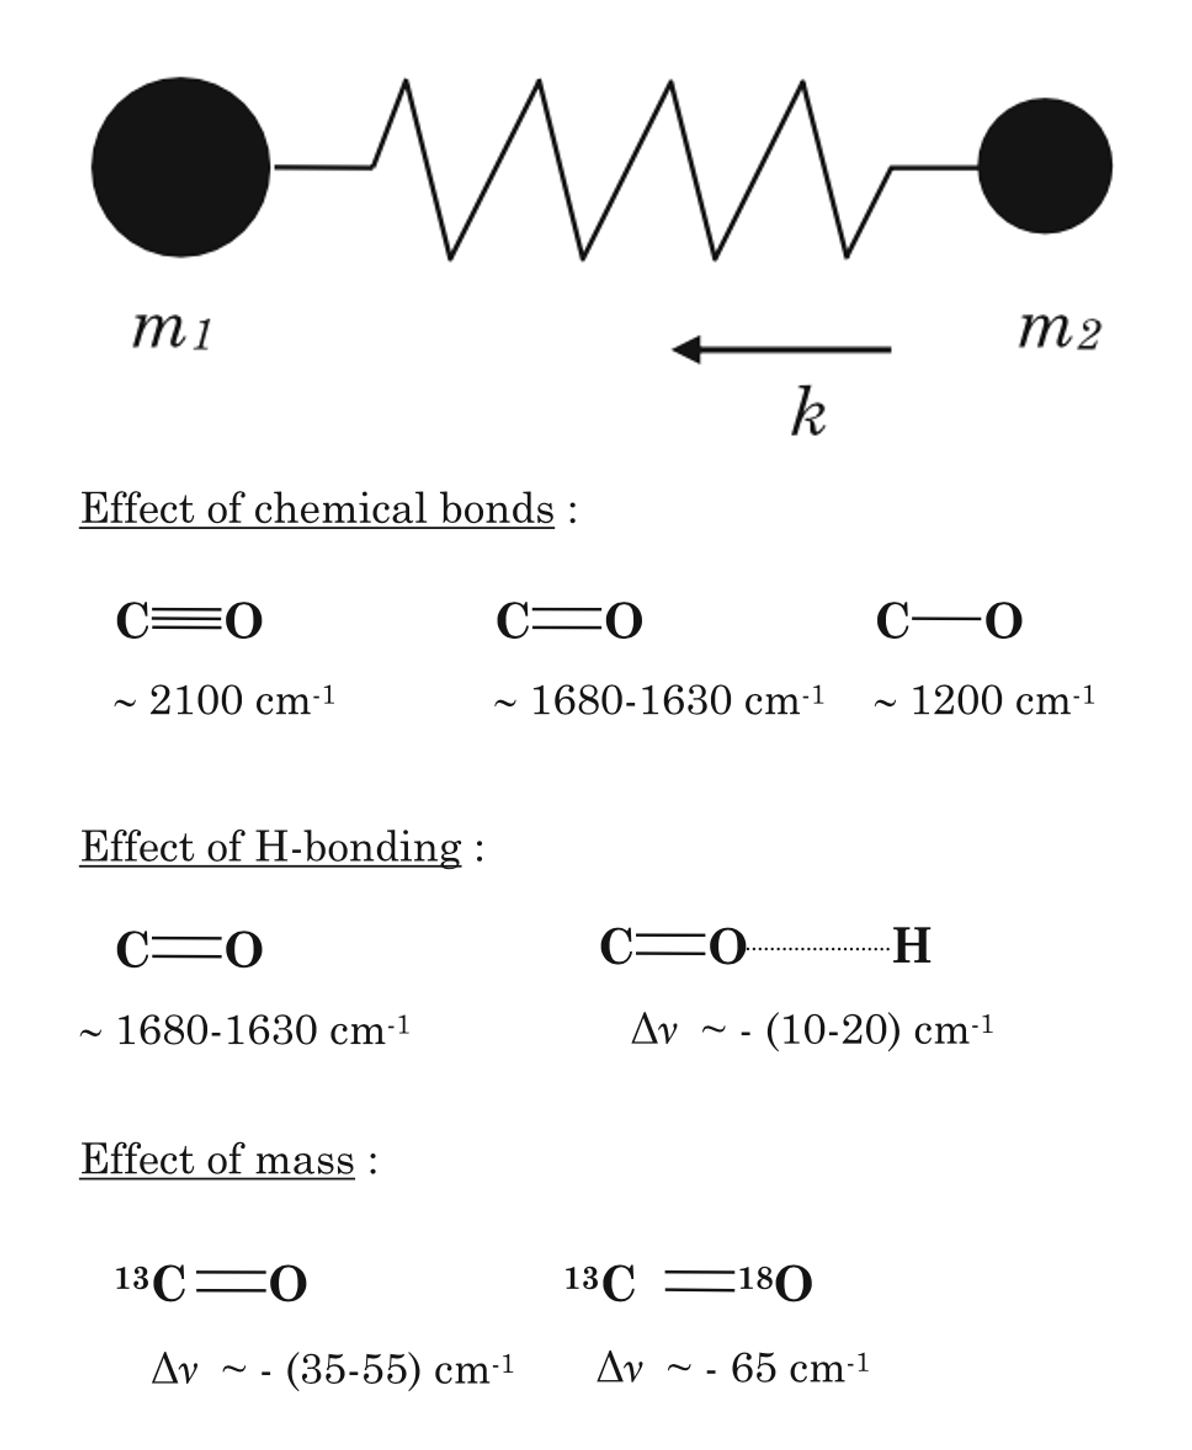
\includegraphics[width=0.8\textwidth]{Images/IR_Basics.png}
  \caption{From \cite{berthomieu_fourier_2009}}
  \label{fig:my-label}
\end{figure}

\begin{figure}[htbp]
  \centering
  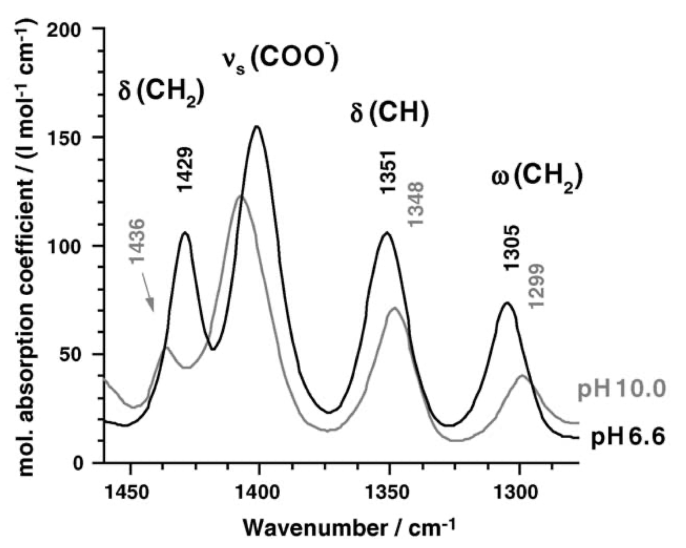
\includegraphics[width=0.8\textwidth]{Images/Cystine_IR_pH_dep.png}
  \caption{From \cite{wolpert_infrared_2006}}
  \label{fig:my-label}
\end{figure}


% \begin{figure}[htbp]
%   \centering
%   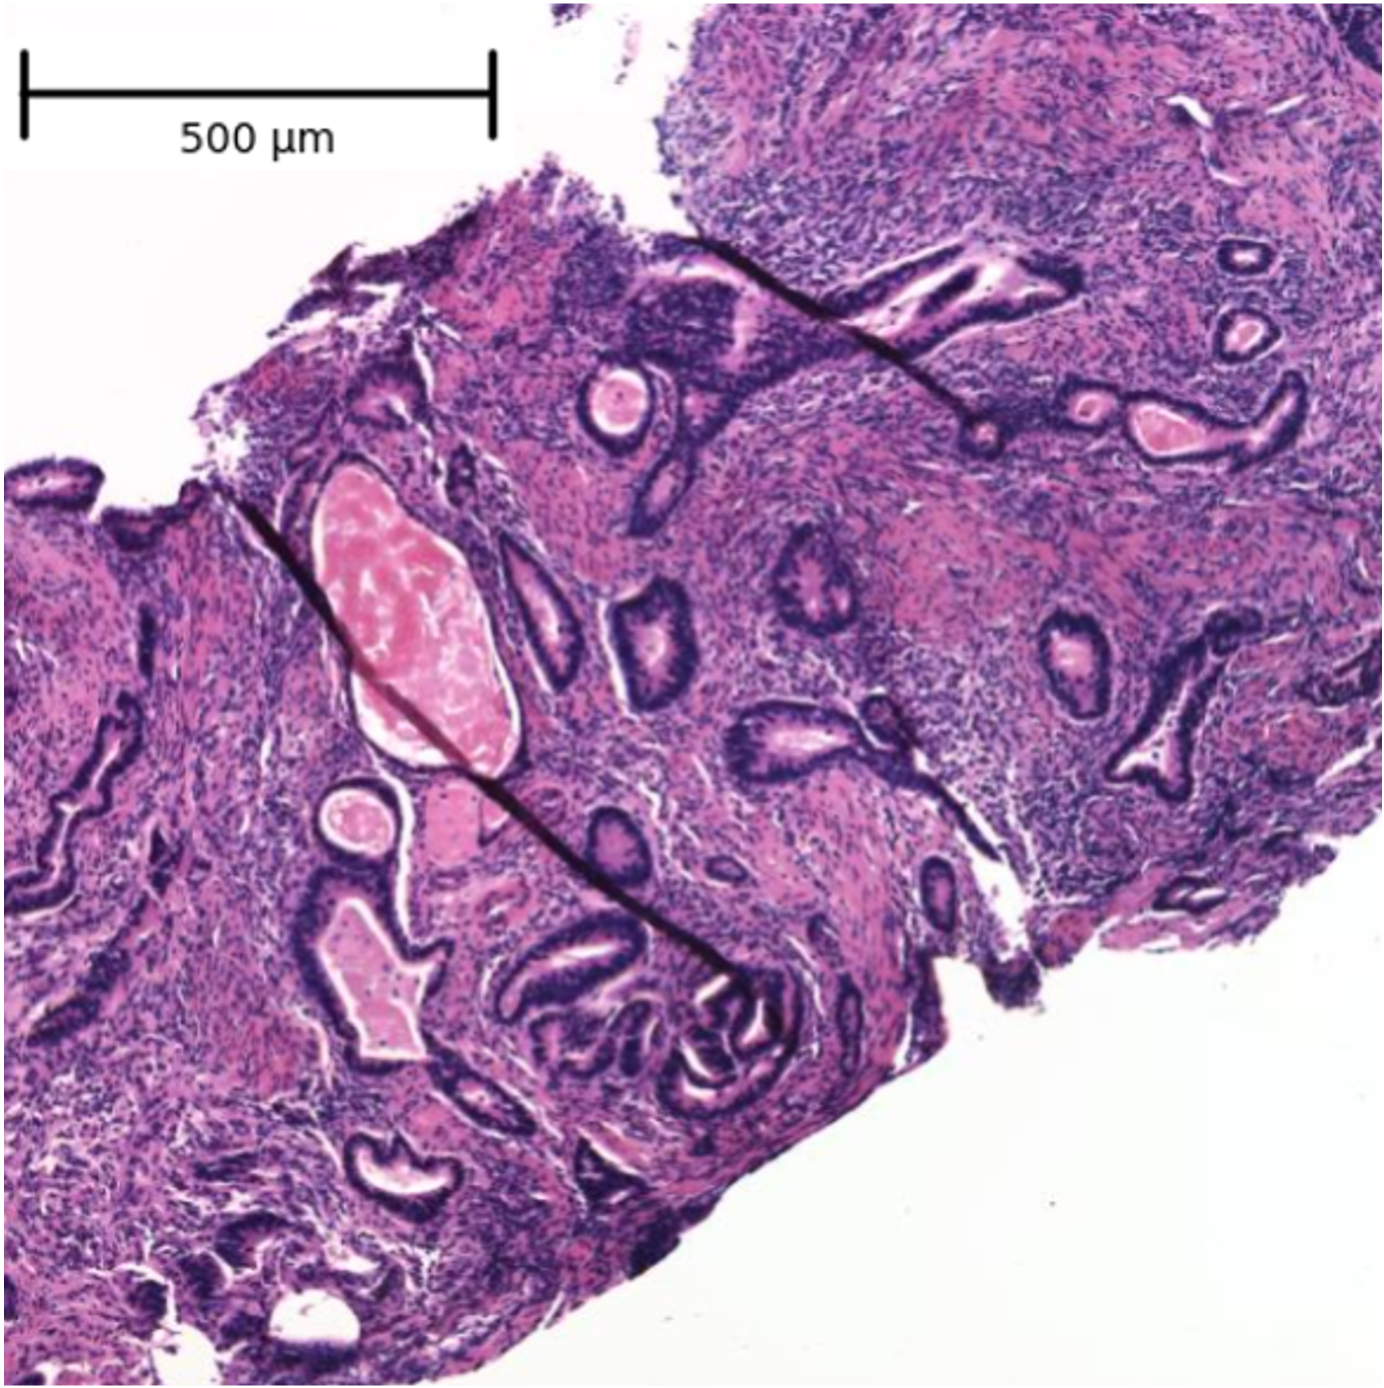
\includegraphics[width=0.8\textwidth]{Images/he_17_scale.png}
%   \caption{Caption}
%   \label{fig:my-label}
% \end{figure}

% \begin{figure}[htbp]
%   \centering
%   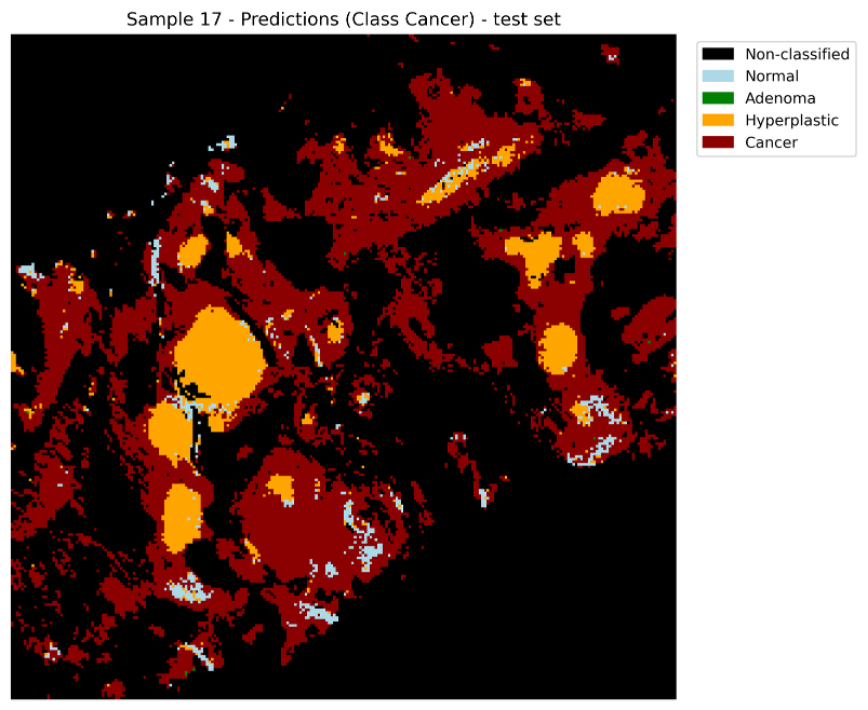
\includegraphics[width=0.8\textwidth]{Images/Predicton_17.png}
%   \caption{Caption}
%   \label{fig:my-label}
% \end{figure}

% \begin{figure}[htbp] 
%     \centering 
%     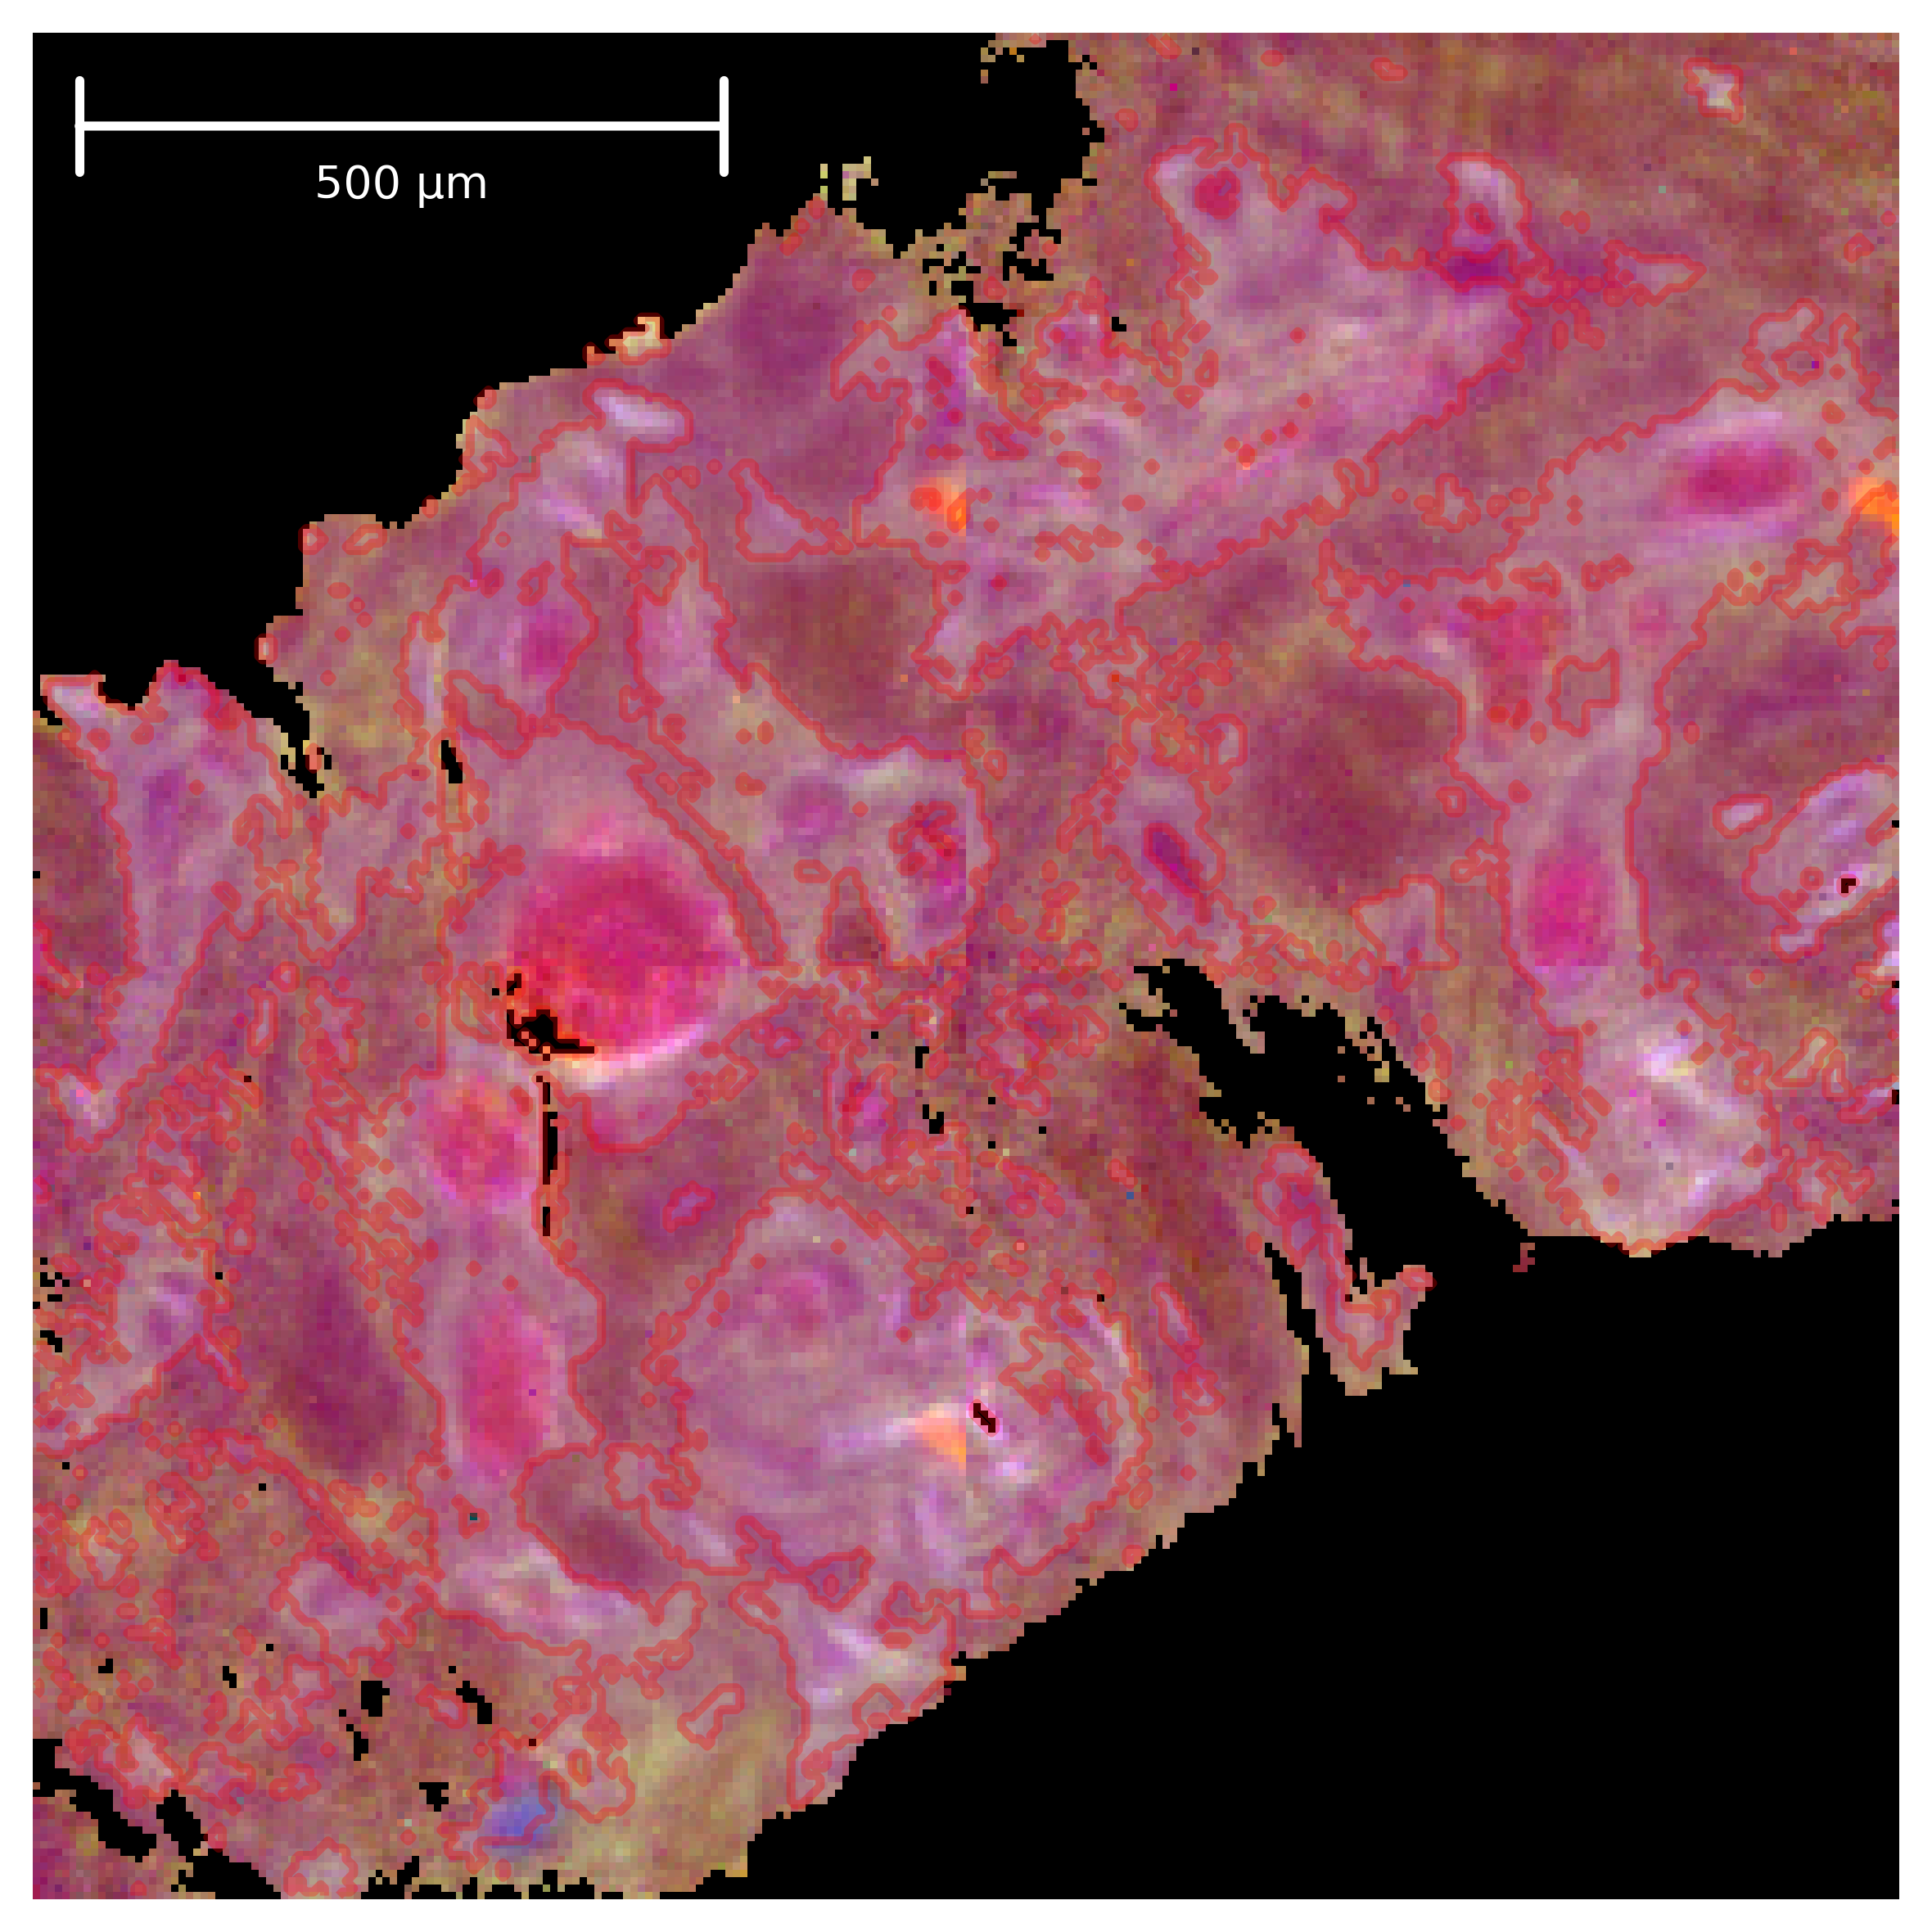
\includegraphics[width=0.8\textwidth]{Images/sample_17_False_IR.png} 
%     \caption{Caption} \label{fig:my-label}
% \end{figure}

% \begin{figure}[htbp] 
%     \centering 
%     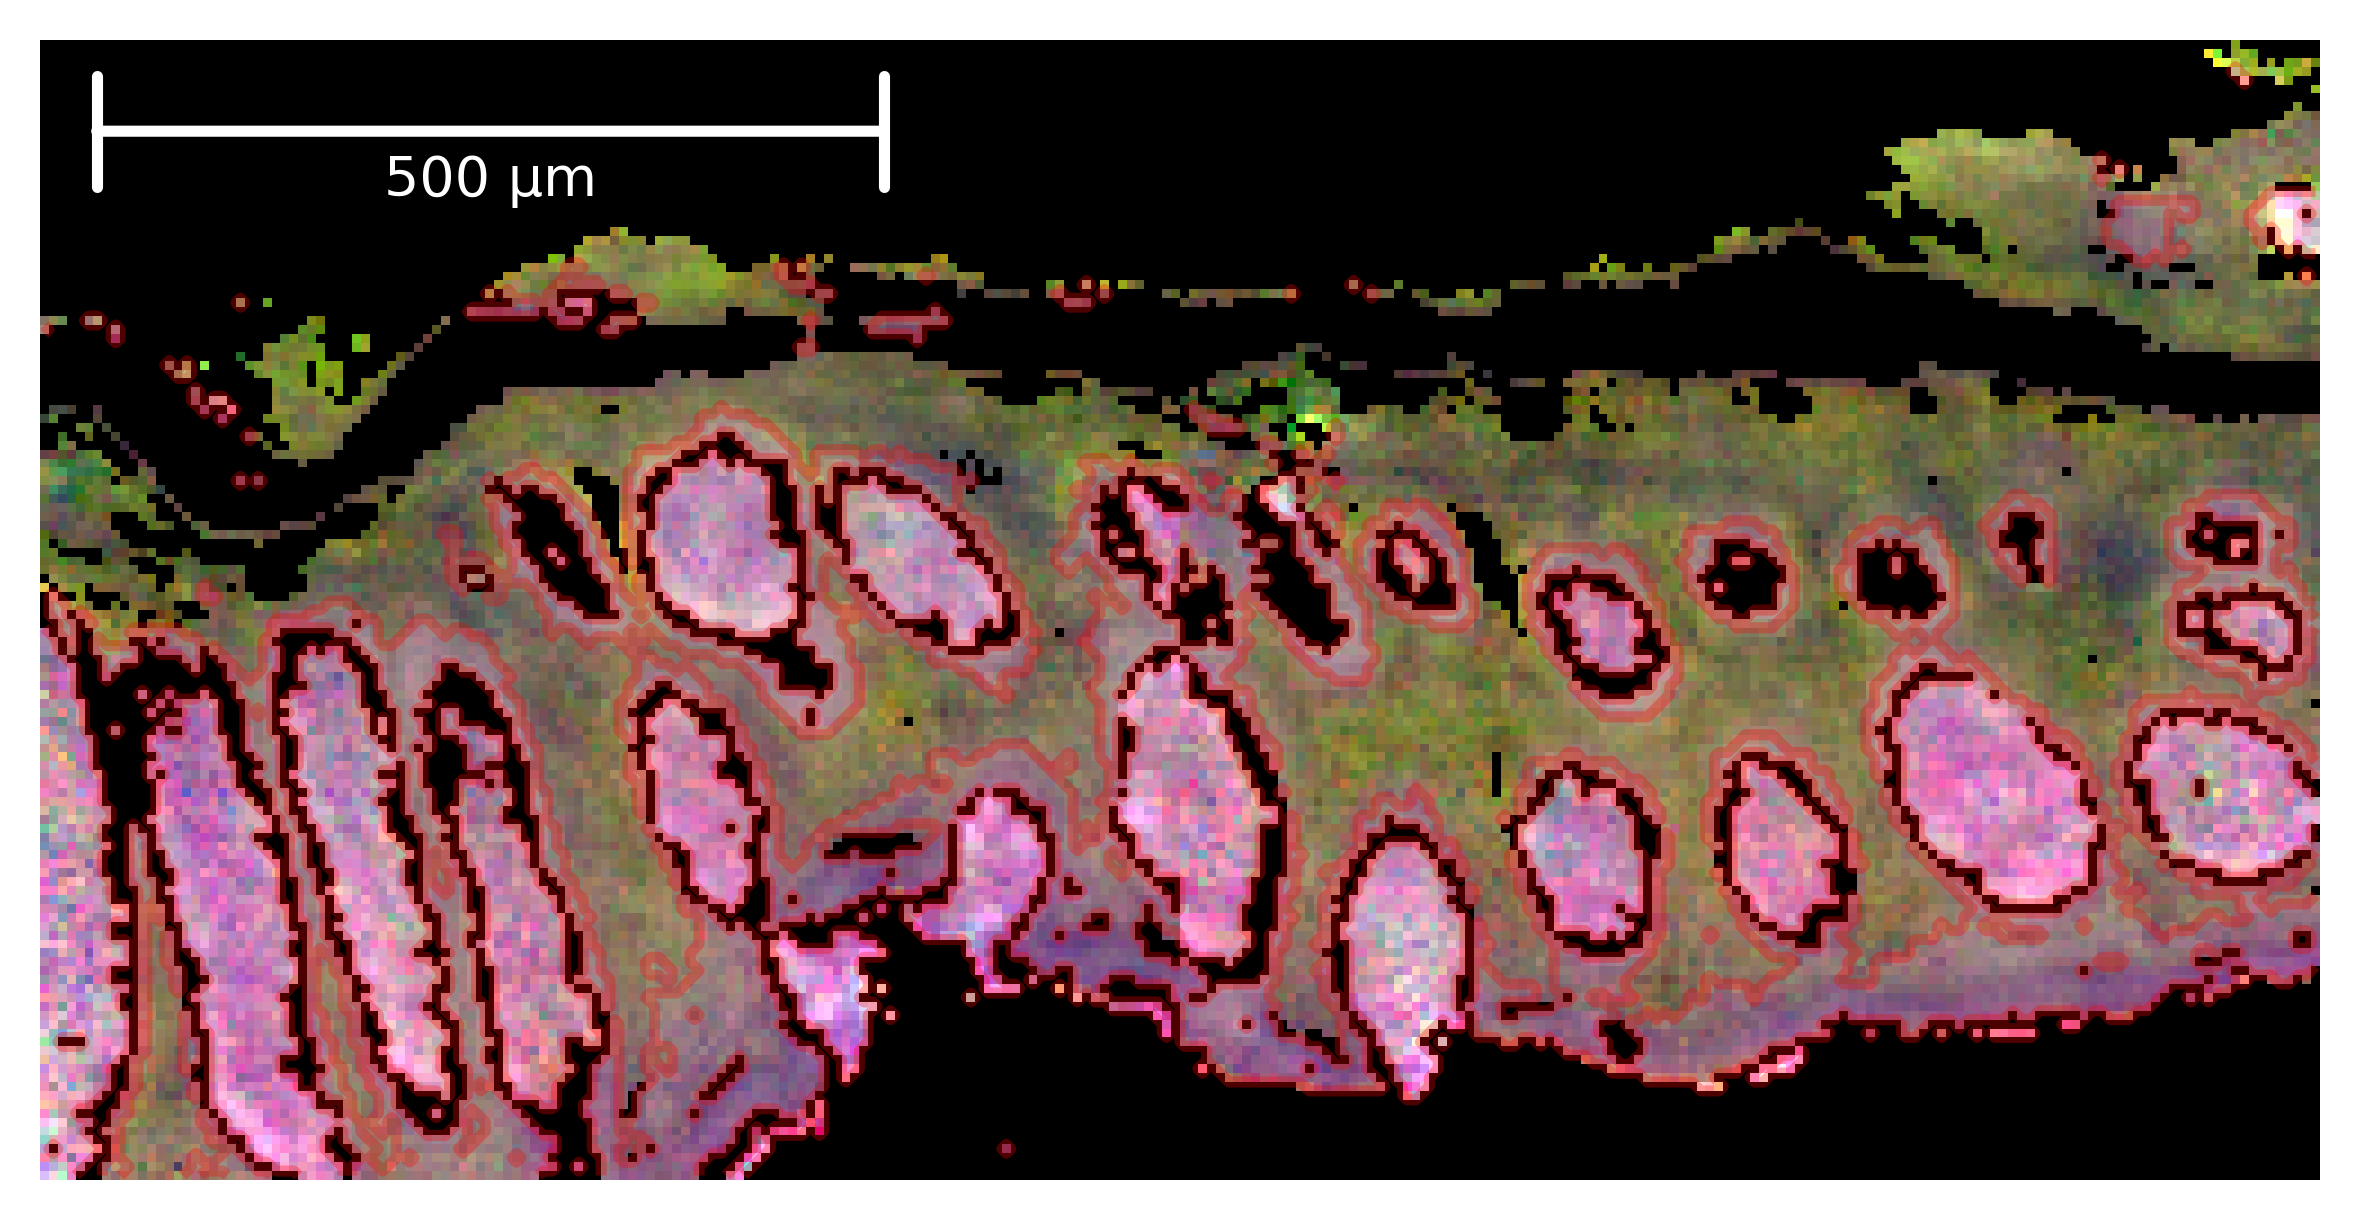
\includegraphics[width=0.8\textwidth]{Images/sample_20_False_IR.png} 
%     \caption{Caption} \label{fig:my-label} 
% \end{figure}

% \begin{figure}[htbp] 
%     \centering 
%     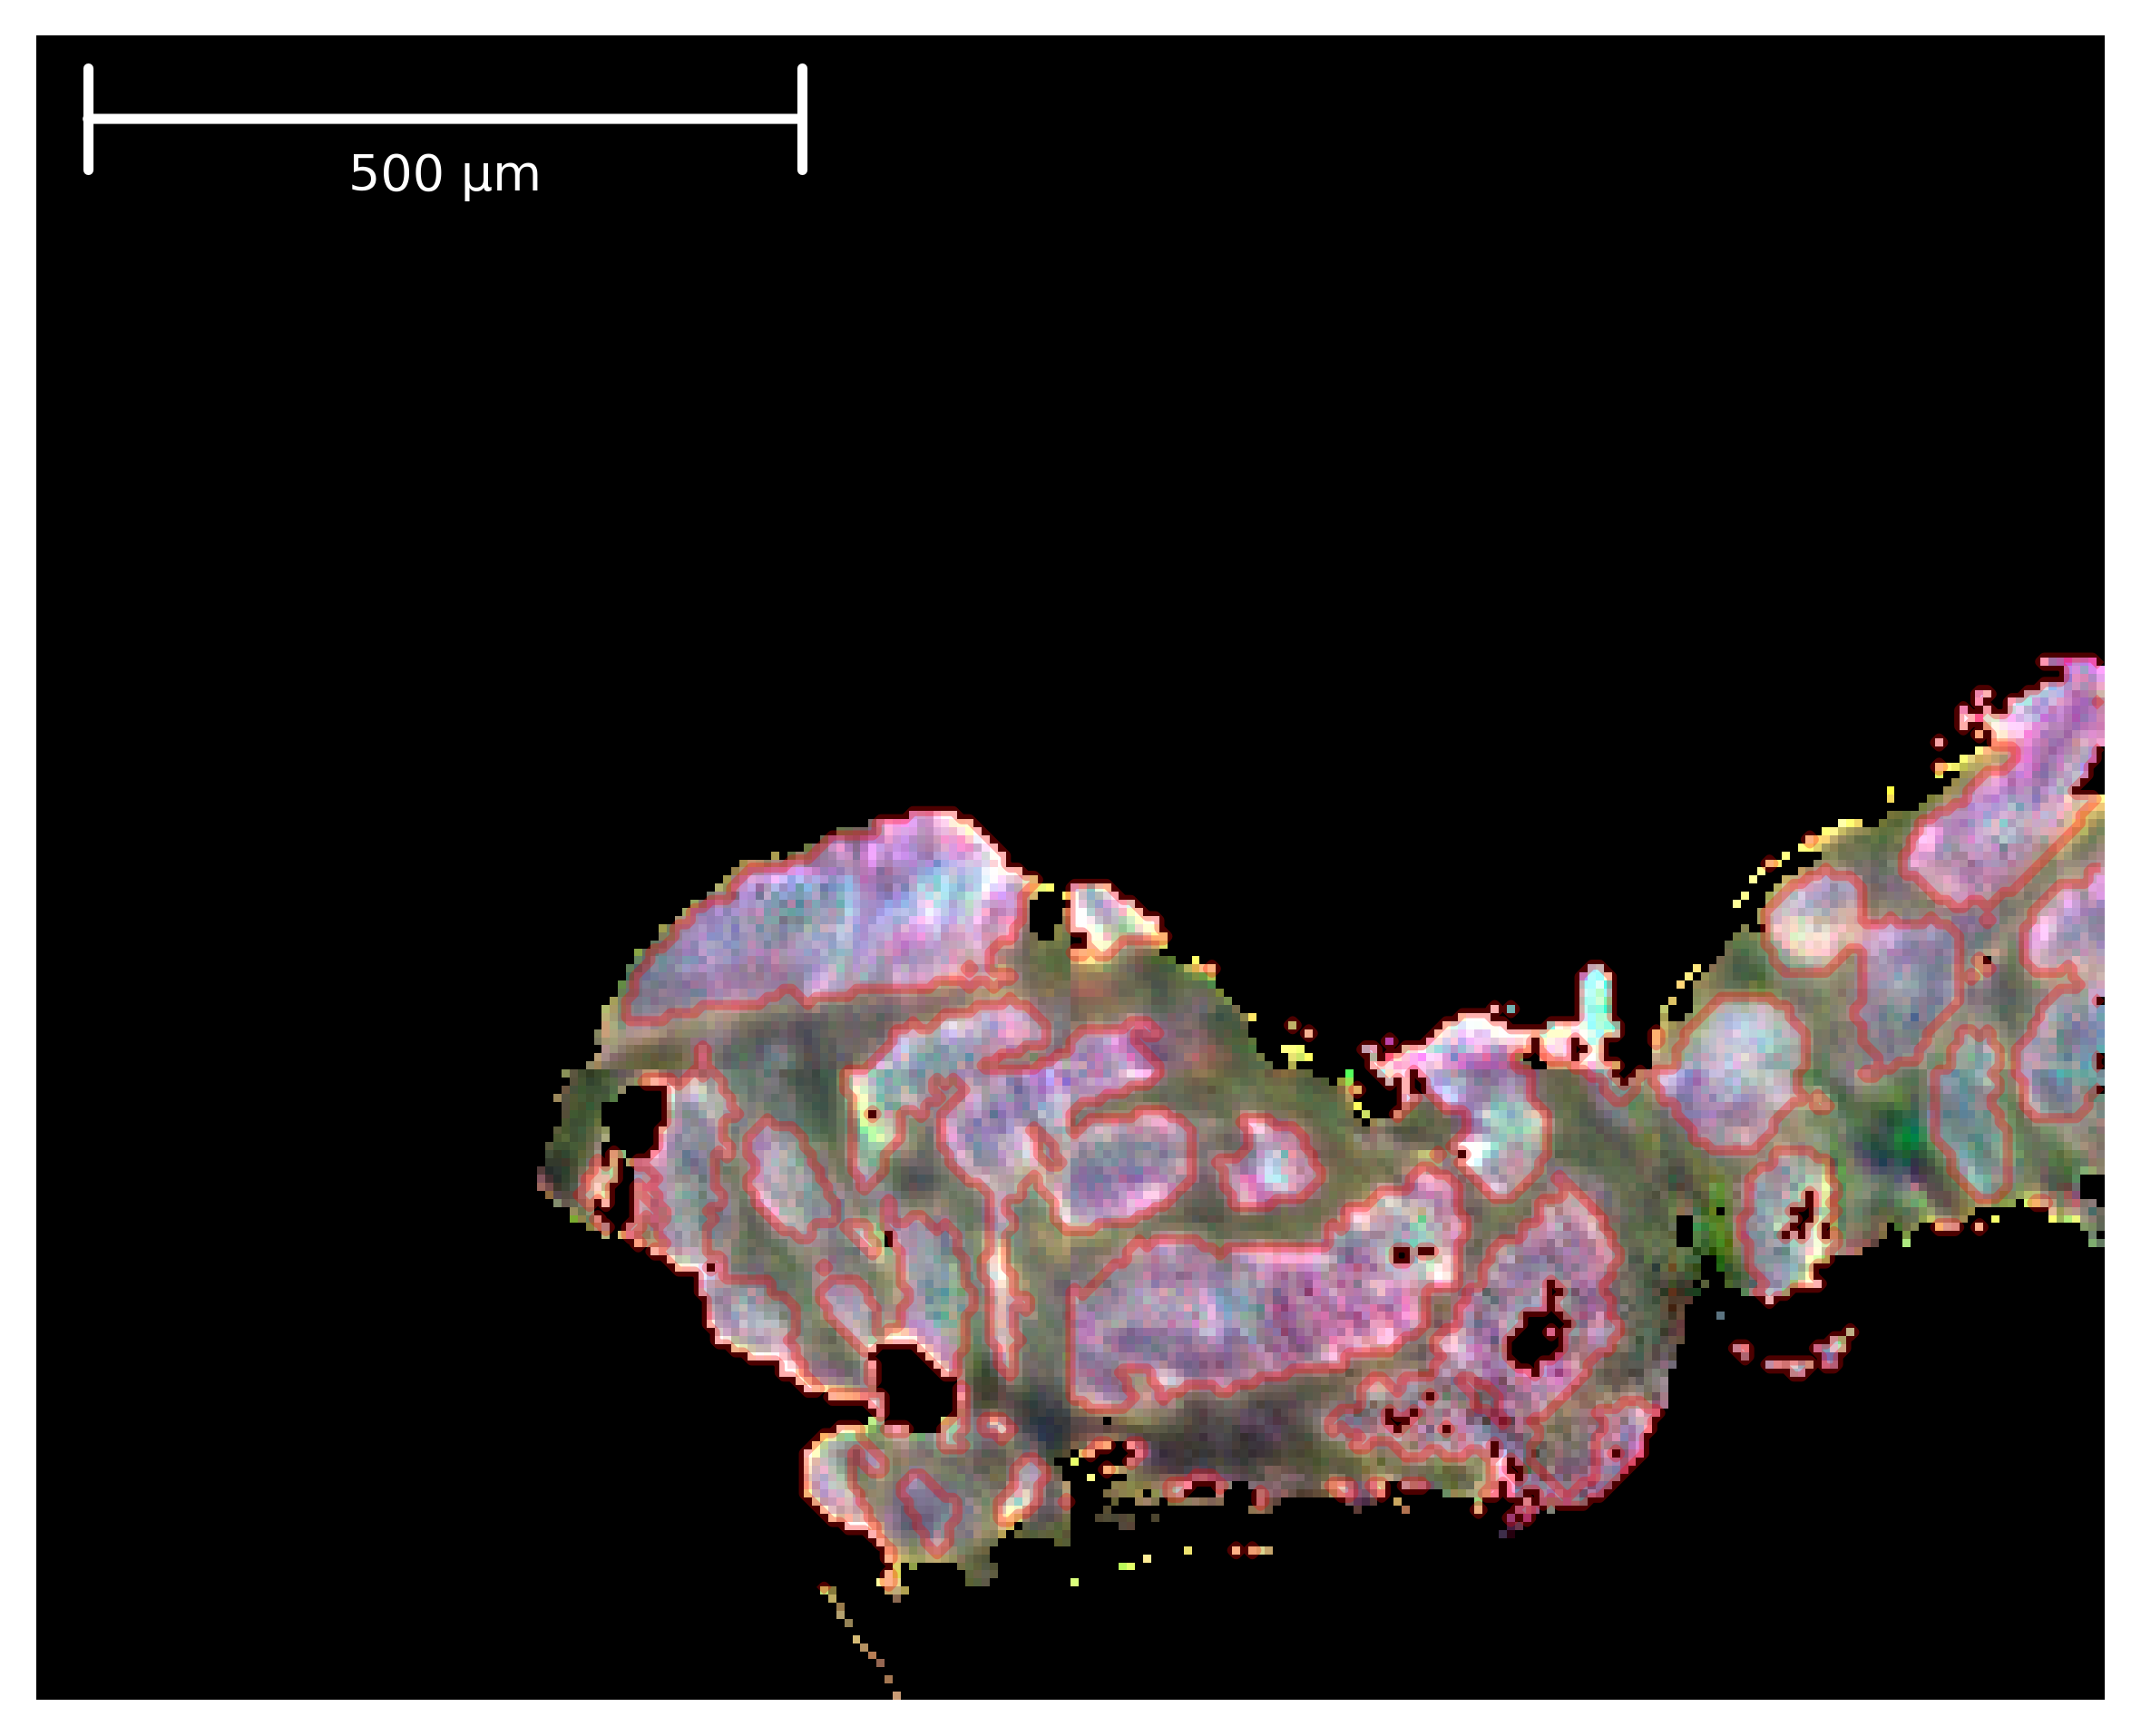
\includegraphics[width=0.8\textwidth]{Images/sample_35_False_IR.png} 
%     \caption{Caption} \label{fig:my-label} 
% \end{figure}

\begin{figure}[htbp] 
    \centering 
    \includegraphics[width=0.9\textwidth]{Images/IR_and_HE_categories.png} 
    \caption{Caption} \label{fig:my-label} 
\end{figure}

\subsubsection{Raman Spectroscopy}
\subsubsection{TPEF}
\subsubsection{SHG}

\subsection{Classical ML Methods for Spectral Classification}

\begin{table}[ht]
  \centering
  \caption{Sensitivity and specificity (mean $\pm$ SD) for each model.}
  \label{tab:model_performance}
  \begin{tabular}{@{}l l c c c c c@{}}
    \toprule
    Model & Metric & Normal & Hyperplastic & Adenoma & Cancer & Accuracy \\
    \midrule
    \multirow{2}{*}{PCA~$>$~LDA}
      & Sensitivity & $42\pm20.4$ & $31\pm17.7$ & $84\pm14.3$ & $39\pm26.3$ & $61\pm7.6$ \\
      & Specificity & $90\pm11.1$ & $94\pm5.4$  & $57\pm19.9$ & $95\pm6.2$  & — \\
    \midrule
    \multirow{2}{*}{XGBoost}
      & Sensitivity & $58\pm11.9$ & $41\pm14.7$ & $80\pm14.4$ & $62\pm33.6$ & $68\pm10.0$ \\
      & Specificity & $88\pm6.6$  & $91\pm2.6$  & $77\pm10.2$ & $96\pm6.2$  & — \\
    \midrule
    \multirow{2}{*}{PCA~$>$~XGBoost}
      & Sensitivity & $43\pm11.5$ & $28\pm11.9$ & $55\pm11.9$ & $75\pm20.9$ & $51\pm9.2$ \\
      & Specificity & $88\pm10.3$ & $90\pm6.7$  & $79\pm7.7$  & $77\pm10.5$ & — \\
    \bottomrule
  \end{tabular}
\end{table}


% Include the other methods here
\subsubsection{XGBoost}
\subsubsection{Spectral Matching}


\subsection{Deep Learning Methods for Spectral Classification}
\subsubsection{Dataset Challenges}
\begin{figure}[htbp]
  \centering
  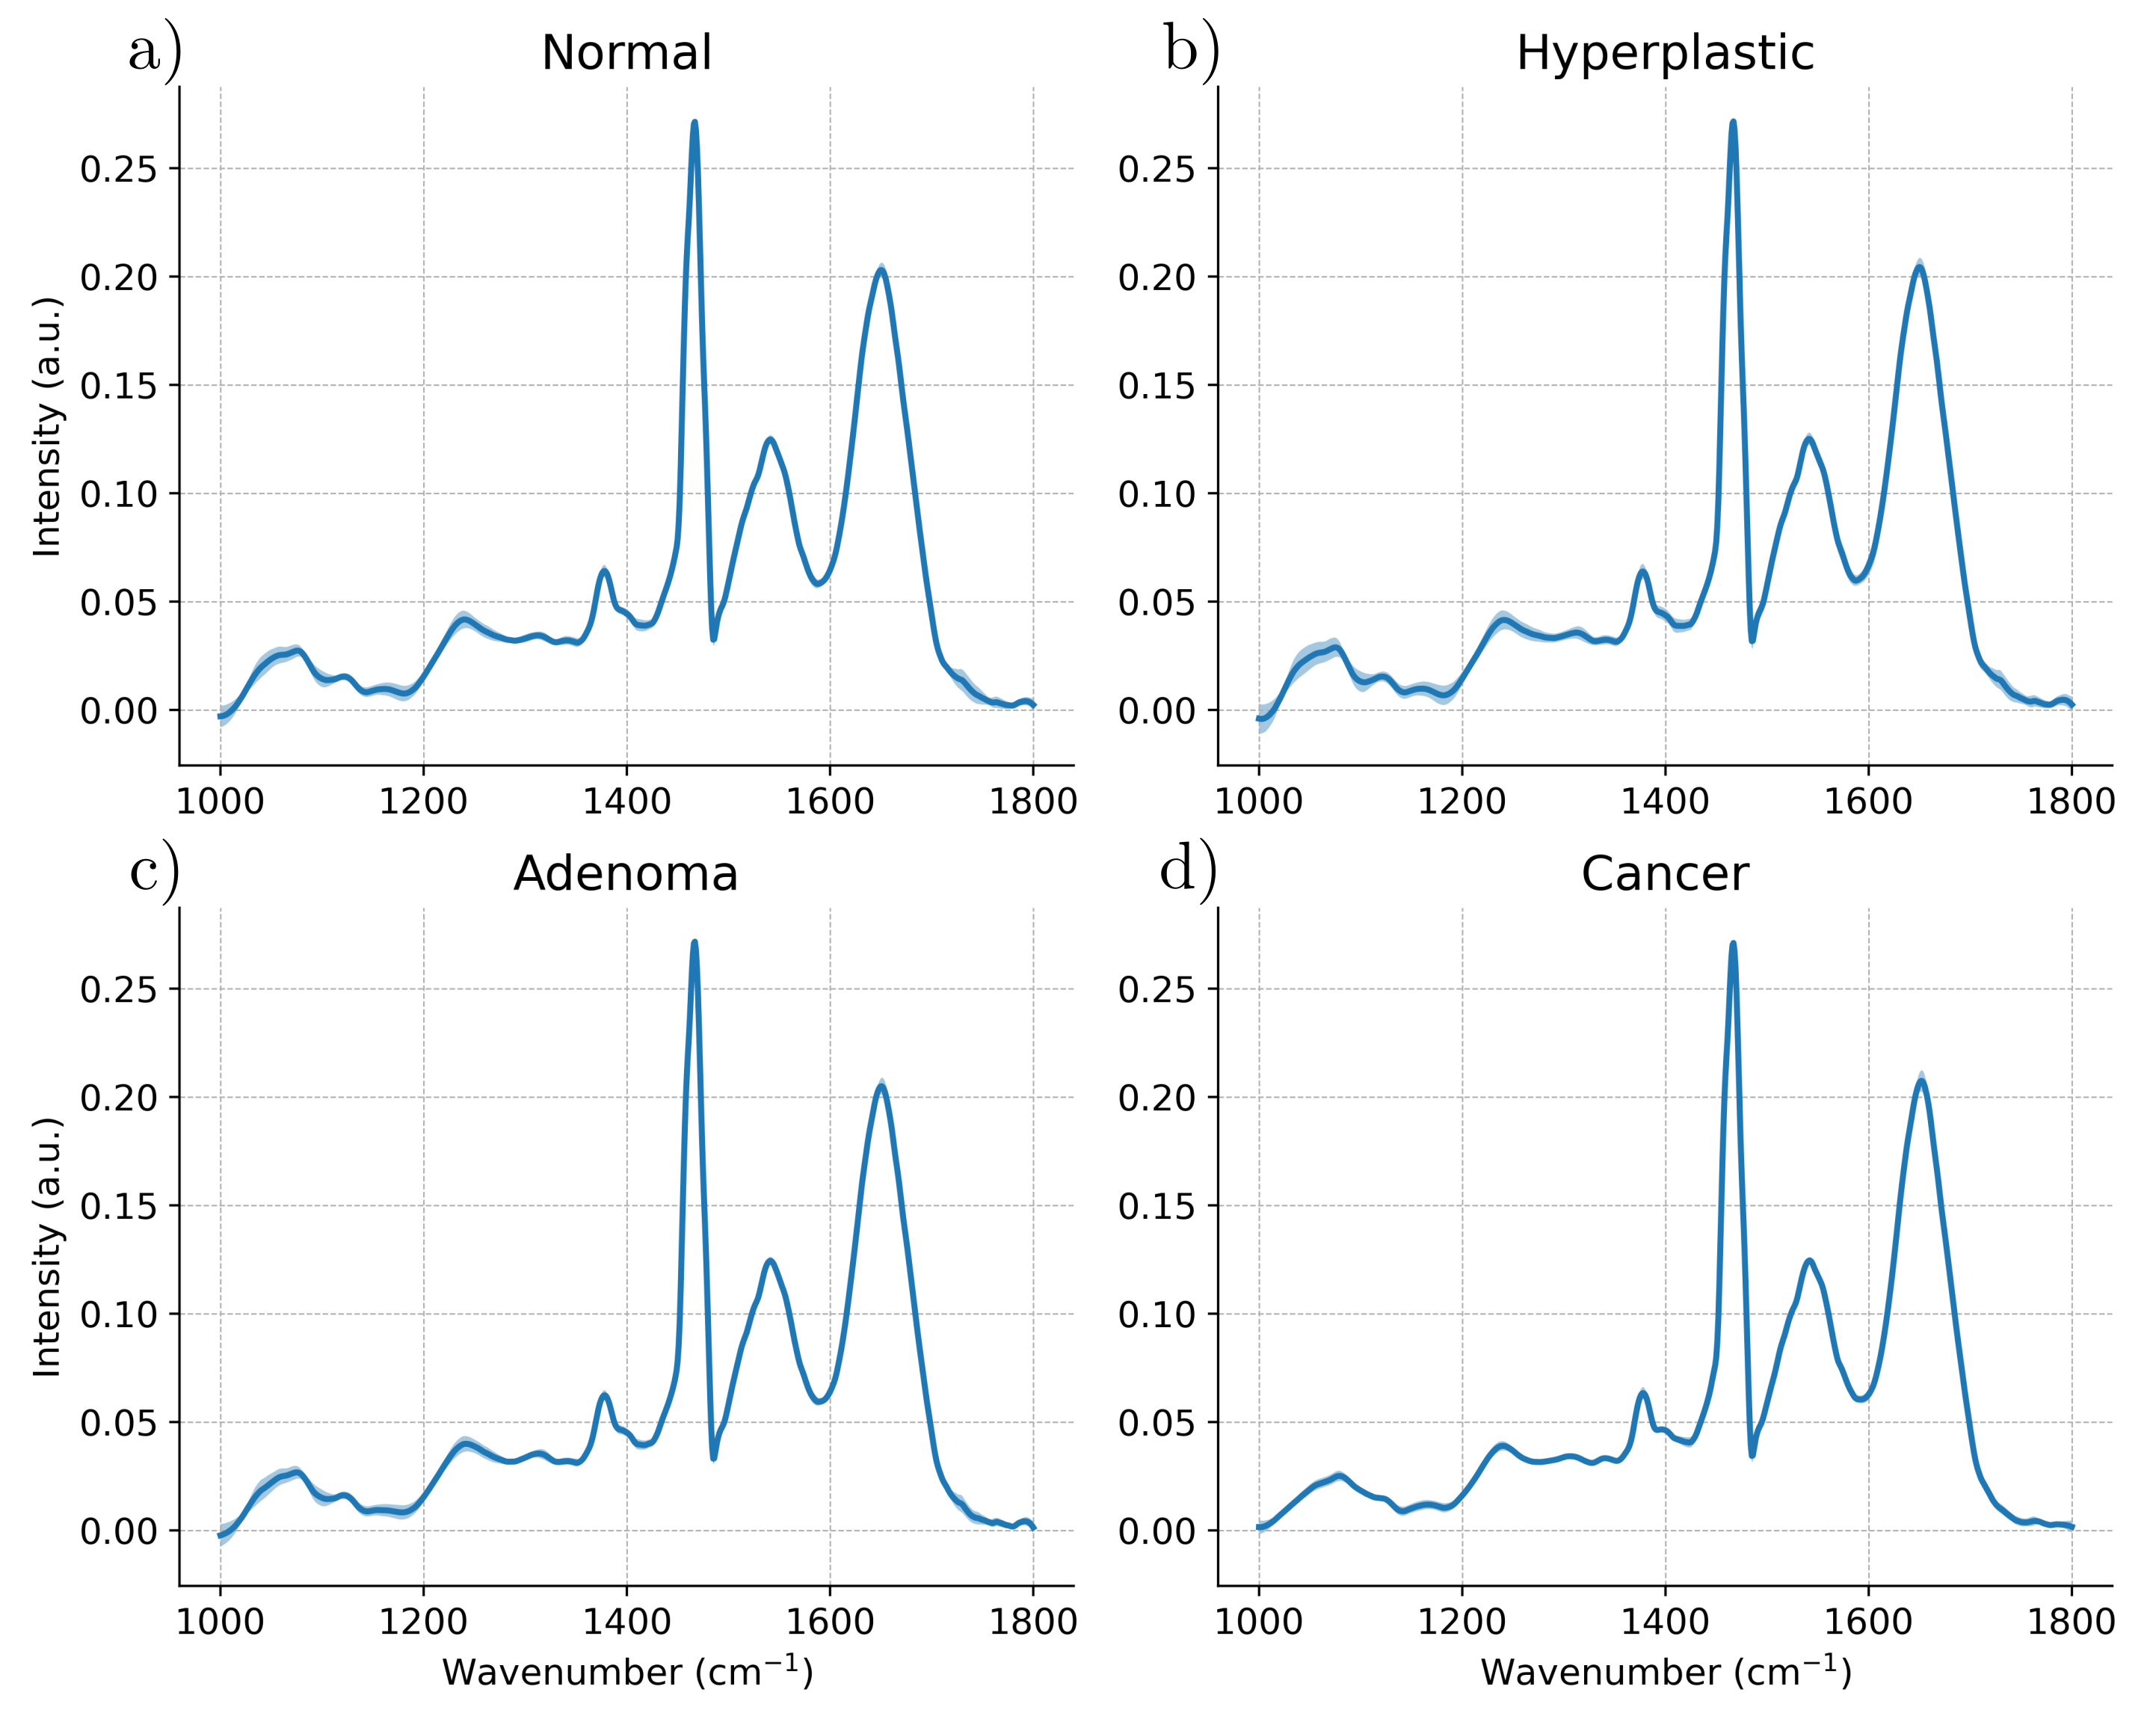
\includegraphics[width=1\textwidth]{Images/Dataset_Class_Differences.png}
  \caption{Caption}
  \label{fig:my-label}
\end{figure}

\subsubsection{De-noising Methods}
\subsubsection{Evaluation Metrics}

\subsubsection{Model Architecture}
\begin{figure}[htbp]
  \centering
  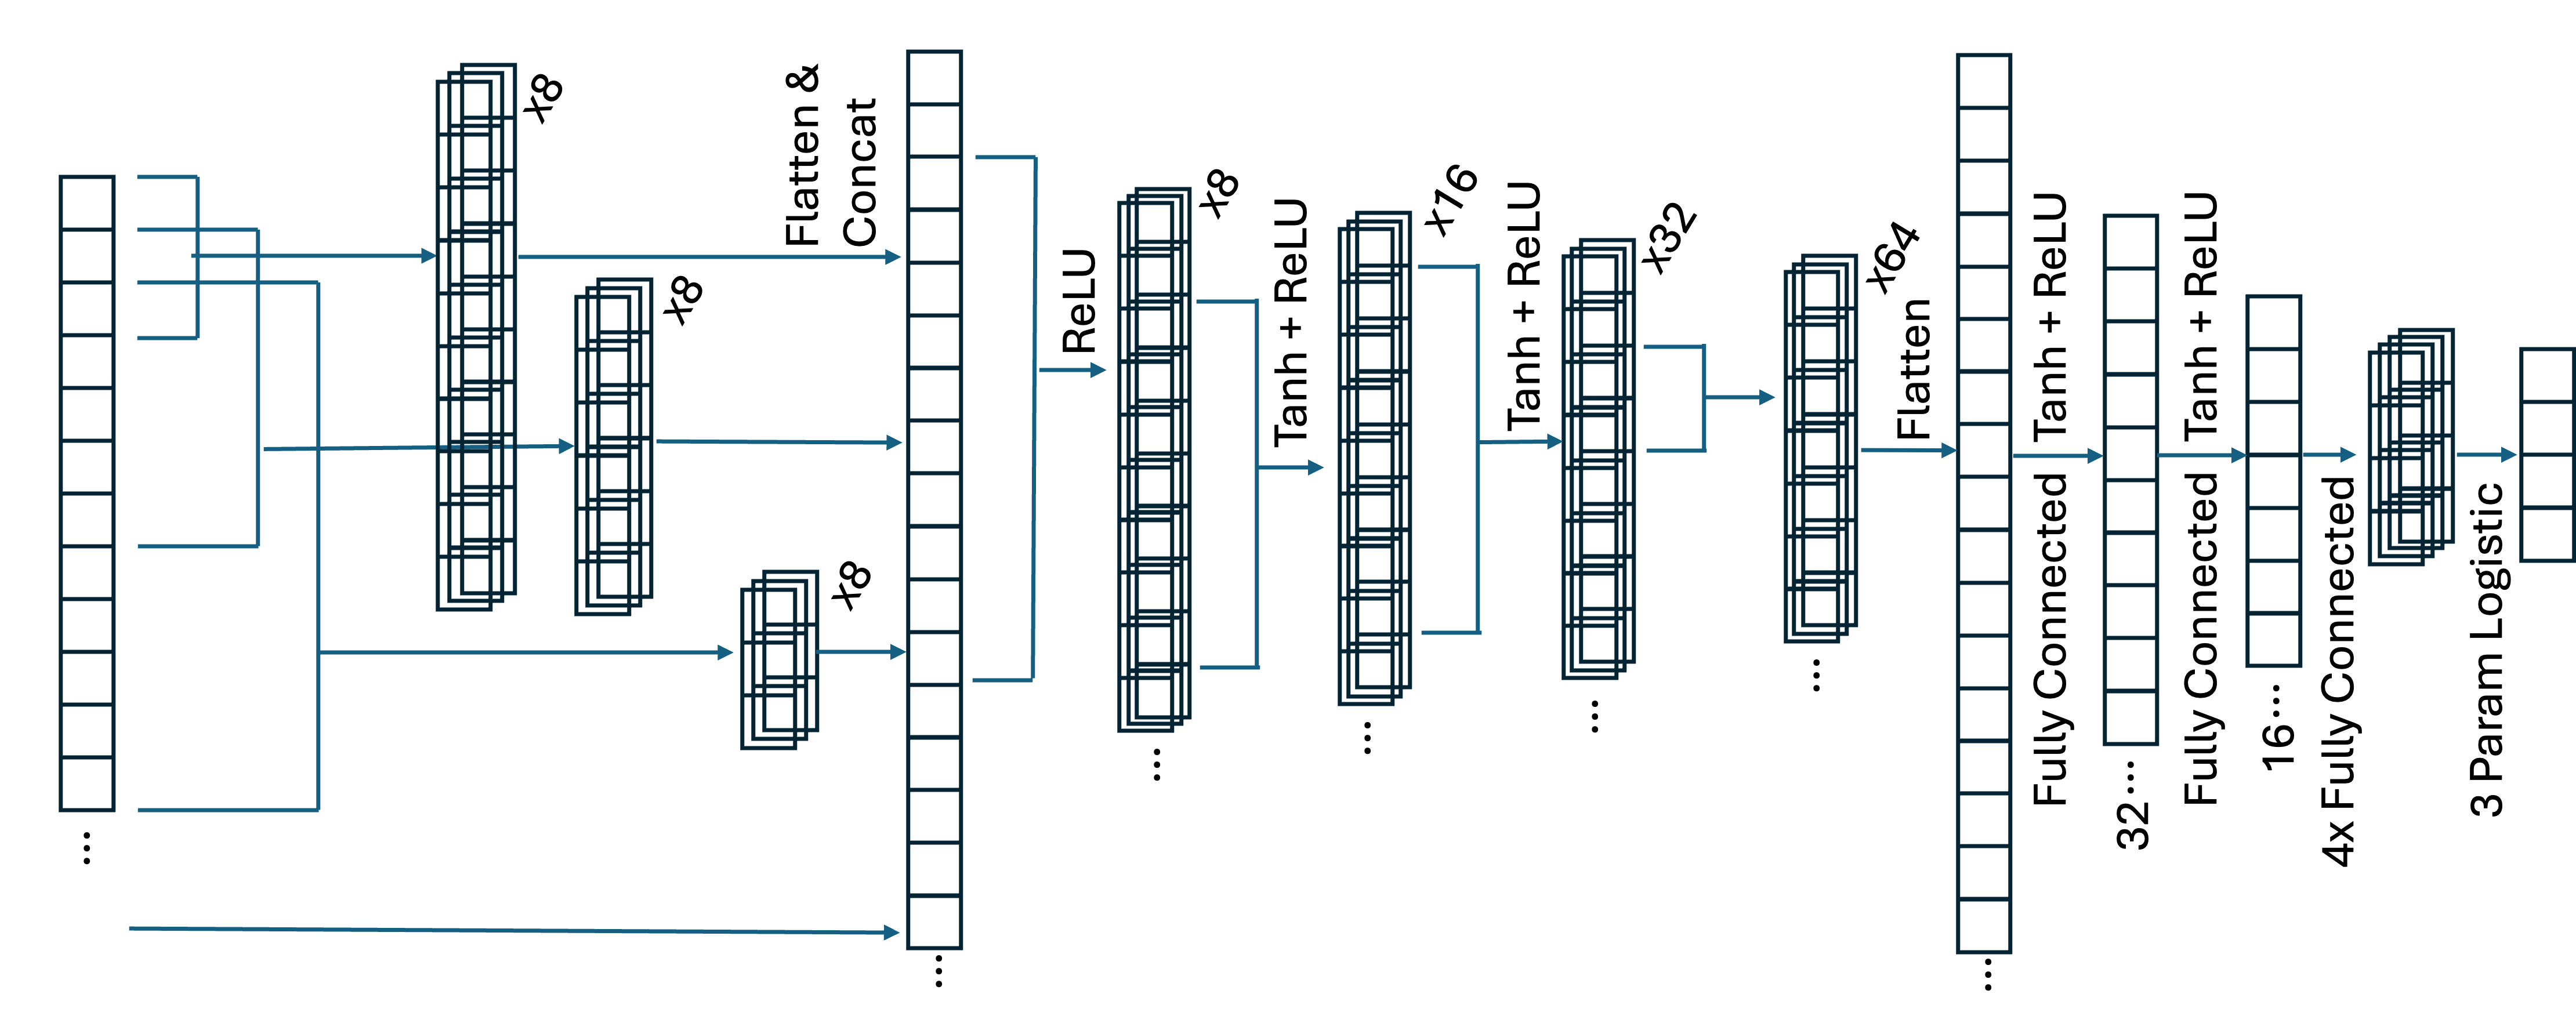
\includegraphics[width=1\textwidth]{Images/SCNN_TPL_Arch.png}
  \caption{Caption}
  \label{fig:my-label}
\end{figure}

\begin{figure}[htbp]
  \centering
  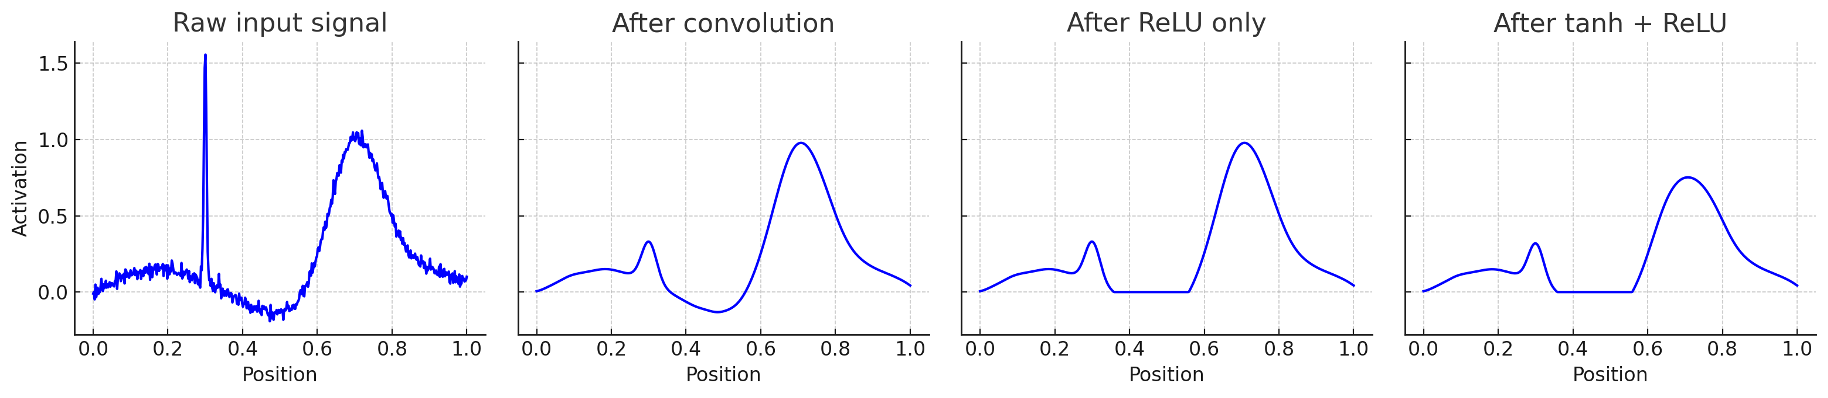
\includegraphics[width=1\textwidth]{Images/Tanh_Relu_Demo.png}
  \caption{Caption}
  \label{fig:my-label}
\end{figure}
\subsubsection{Regularisation Techniques}

\begin{figure}[htbp] 
    \centering 
    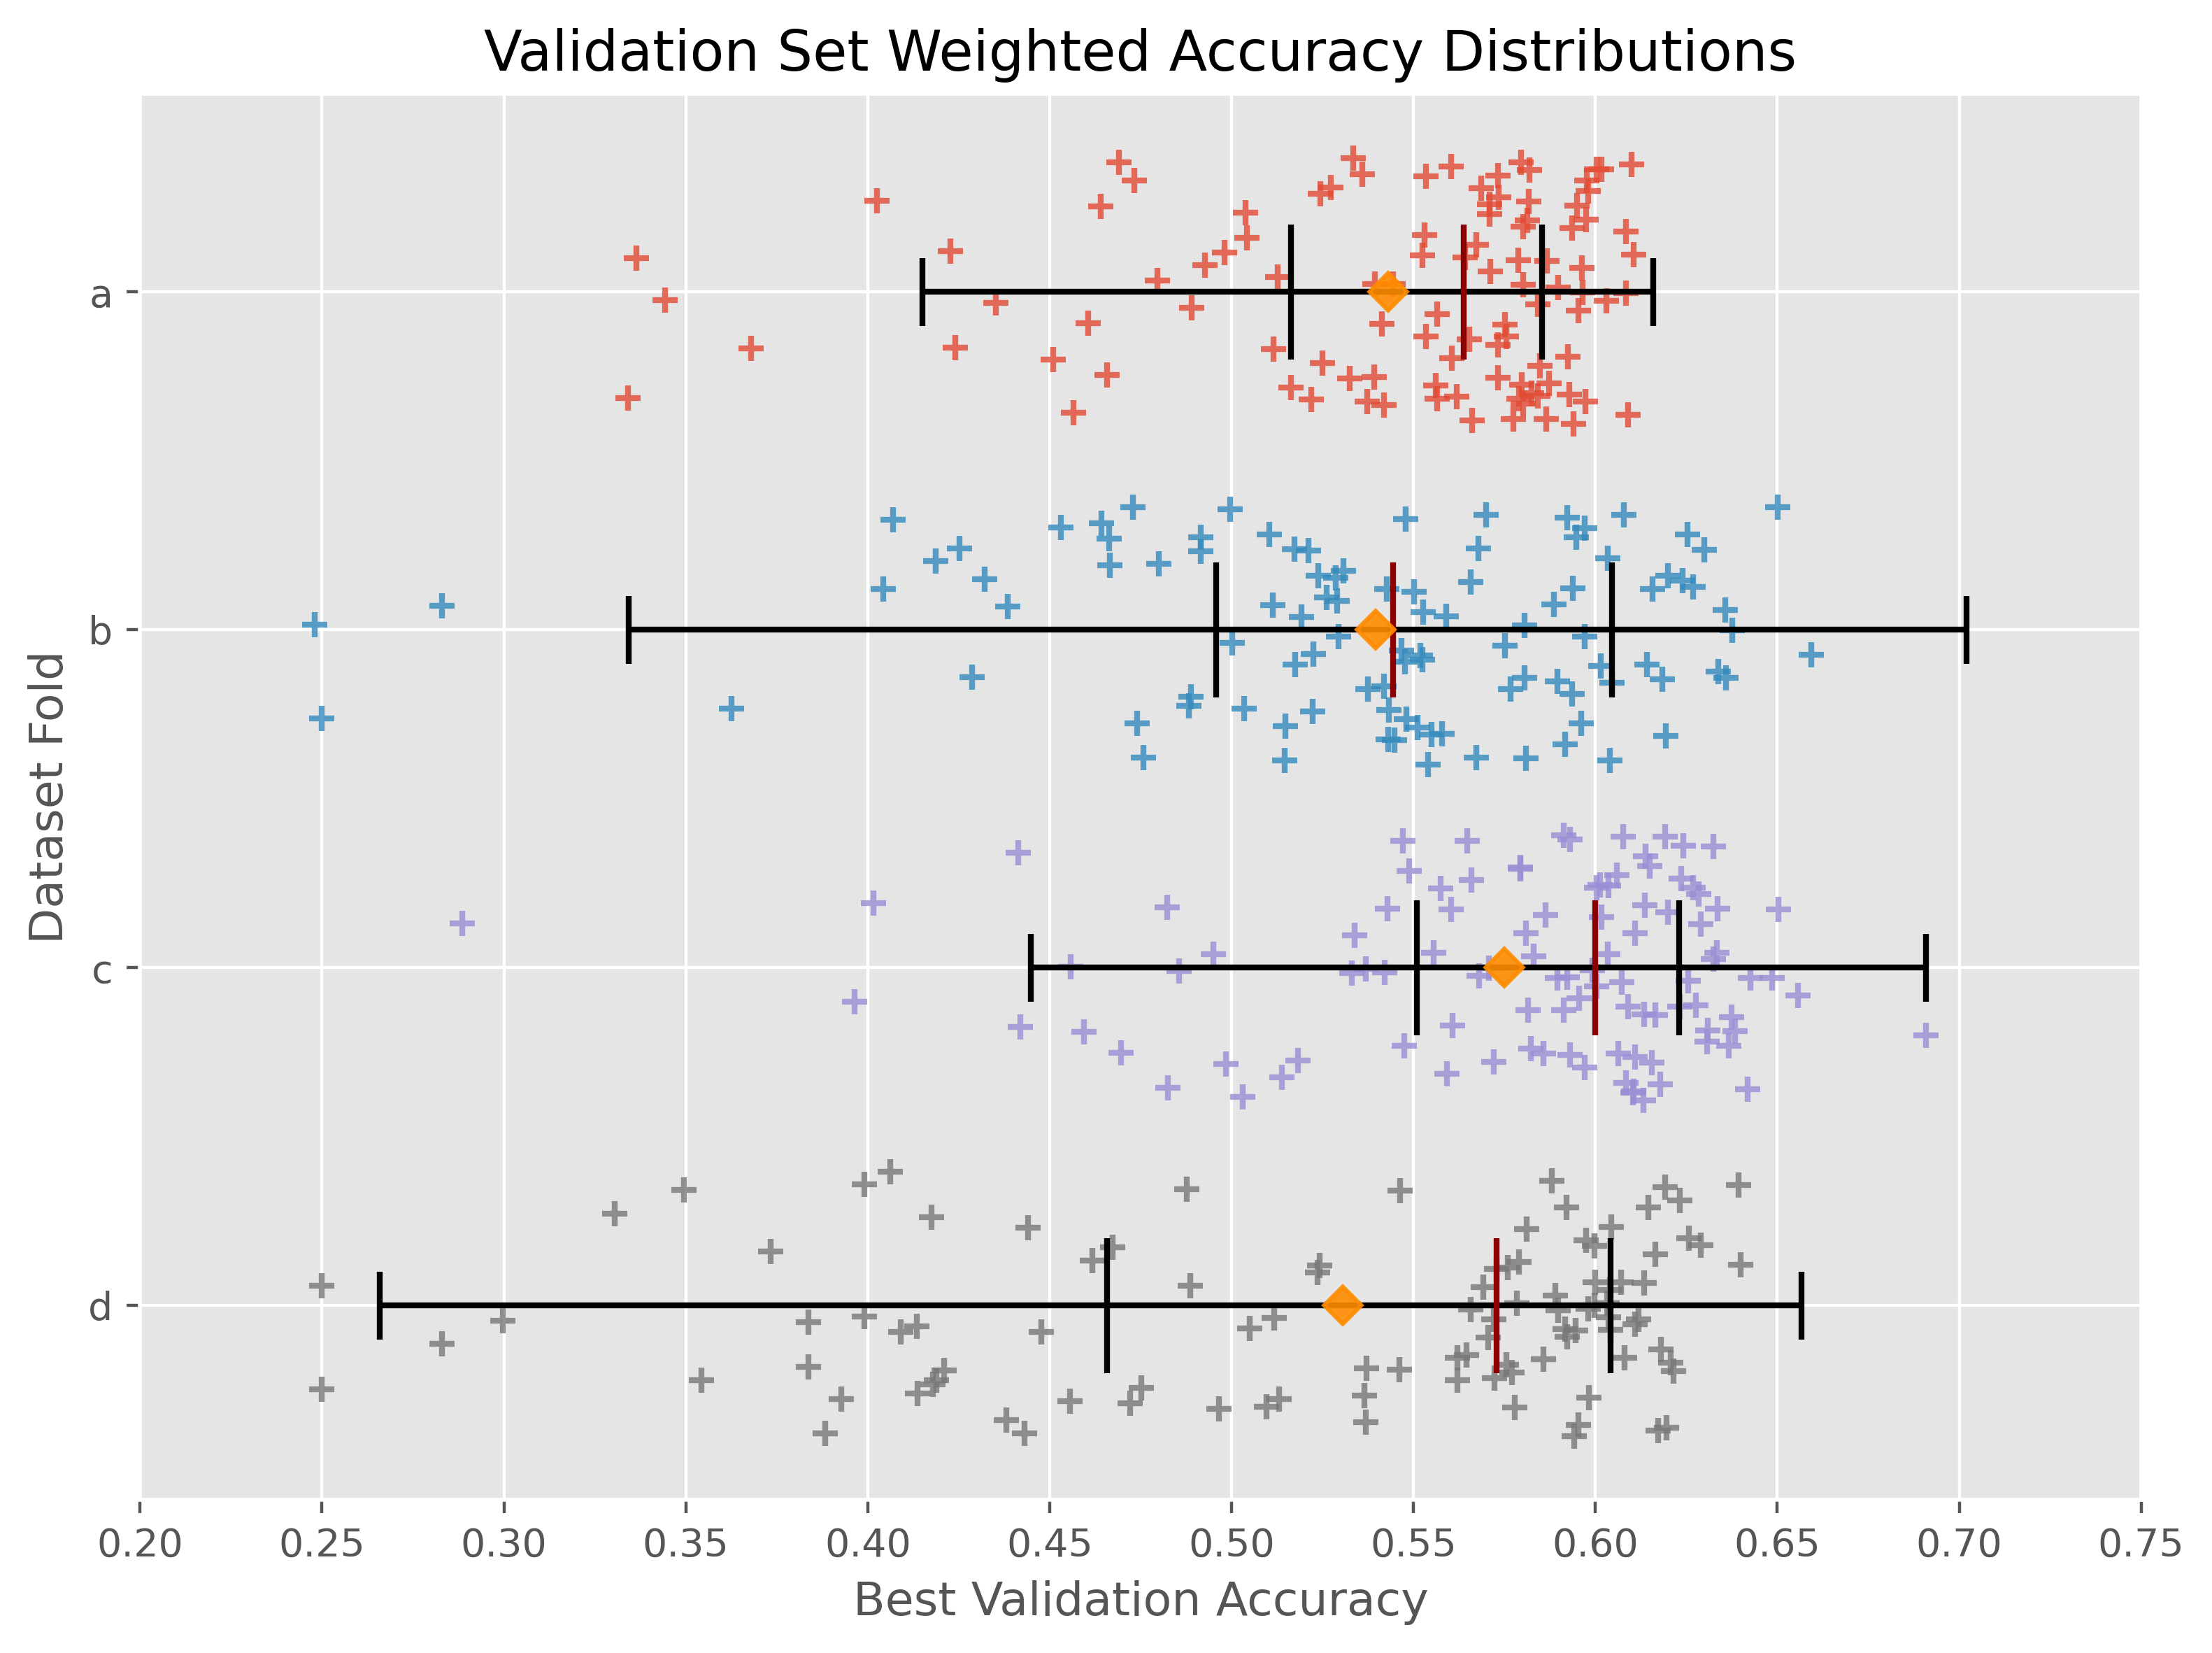
\includegraphics[width=1\textwidth]{Images/best_val_accuracy.png} 
    \caption{Caption} \label{fig:my-label}
\end{figure}

\begin{table}[ht] \centering \caption{Metrics for single fold test set
with 50\% voting threshold and no label smoothing} \begin{tabular}{lcccc} \toprule Metrics & Normal & Hyperplastic & Adenoma & Cancer \\
\midrule
Accuracy & $0.699$ & $0.680$ & $0.699$ & $0.945$ \\
Sensitivity & $0.662$ & $0.258$ & $0.452$ & $0.783$ \\
Specificity & $0.708$ & $0.762$ & $0.936$ & $0.972$ \\
False Positive Rate & $0.292$ & $0.238$ & $0.064$ & $0.028$ \\
\midrule \multicolumn{5}{c}{\textbf{Overall Weighted Accuracy:} $0.5387$} \\
\bottomrule \end{tabular}
\label{tab:voting05_results} \end{table}

\begin{table}[ht] \centering \caption{Metrics for single fold test set with 50\% voting threshold and 10\% label smoothing} \begin{tabular}{lcccc} \toprule Metrics & Normal & Hyperplastic & Adenoma & Cancer \\
\midrule
Accuracy & $0.702$ & $0.674$ & $0.700$ & $0.944$ \\
Sensitivity & $0.643$ & $0.257$ & $0.458$ & $0.782$ \\
Specificity & $0.716$ & $0.755$ & $0.933$ & $0.971$ \\
False Positive Rate & $0.284$ & $0.245$ & $0.067$ & $0.029$ \\
\midrule \multicolumn{5}{c}{\textbf{Overall Weighted Accuracy:} $0.5349$} \\
\bottomrule
\end{tabular} \label{tab:ls01_results} \end{table}

\begin{table}[ht] \centering \caption{Metrics for single fold test set with 50\% voting threshold and 20\% label smoothing} \begin{tabular}{lcccc} \toprule Metrics & Normal & Hyperplastic & Adenoma & Cancer \\
\midrule
Accuracy & $0.700$ & $0.672$ & $0.692$ & $0.941$ \\
Sensitivity & $0.650$ & $0.266$ & $0.436$ & $0.786$ \\
Specificity & $0.713$ & $0.751$ & $0.937$ & $0.967$ \\
False Positive Rate & $0.287$ & $0.249$ & $0.063$ & $0.033$ \\
\midrule \multicolumn{5}{c}{\textbf{Overall Weighted Accuracy:} $0.5345$} \\
\bottomrule
\end{tabular} \label{tab:ls02_results} \end{table}


\subsubsection{Model Performance}

\begin{figure}[htbp] 
    \centering 
    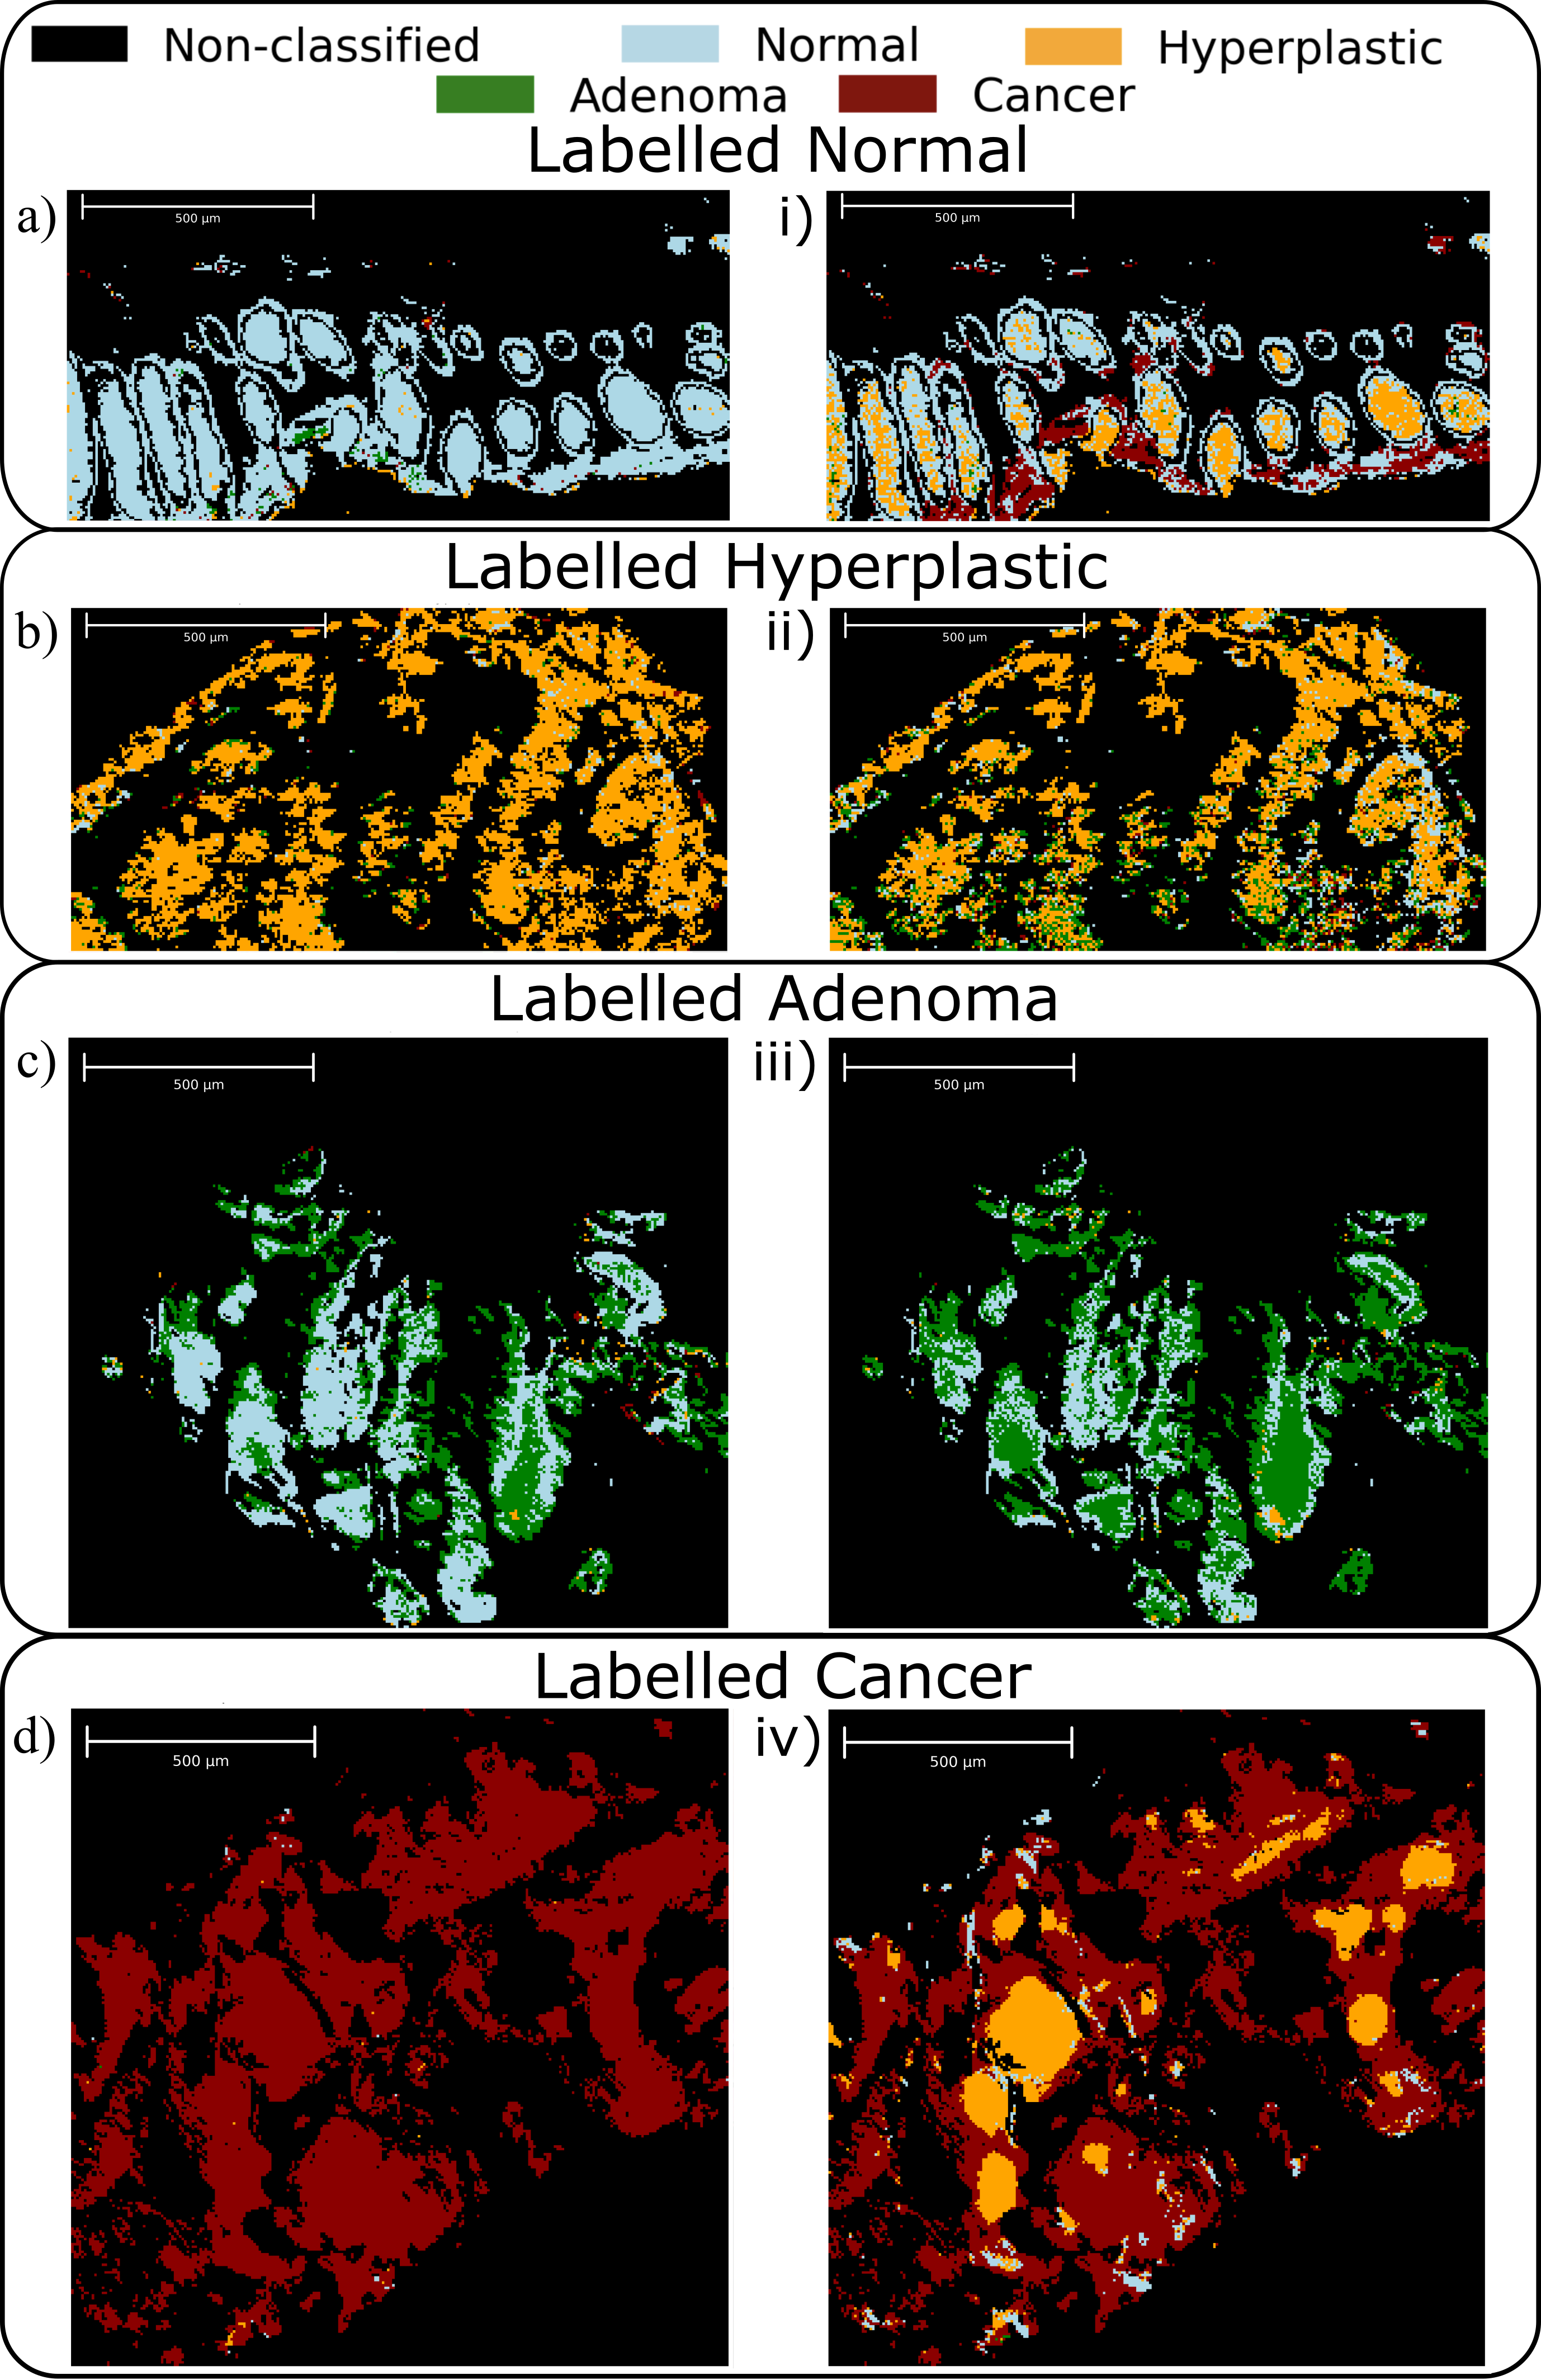
\includegraphics[width=0.8\textwidth]{Images/Categorisation_train_test.png} 
    \caption{Caption} \label{fig:my-label} 
\end{figure}

\begin{figure}[htbp] 
    \centering 
    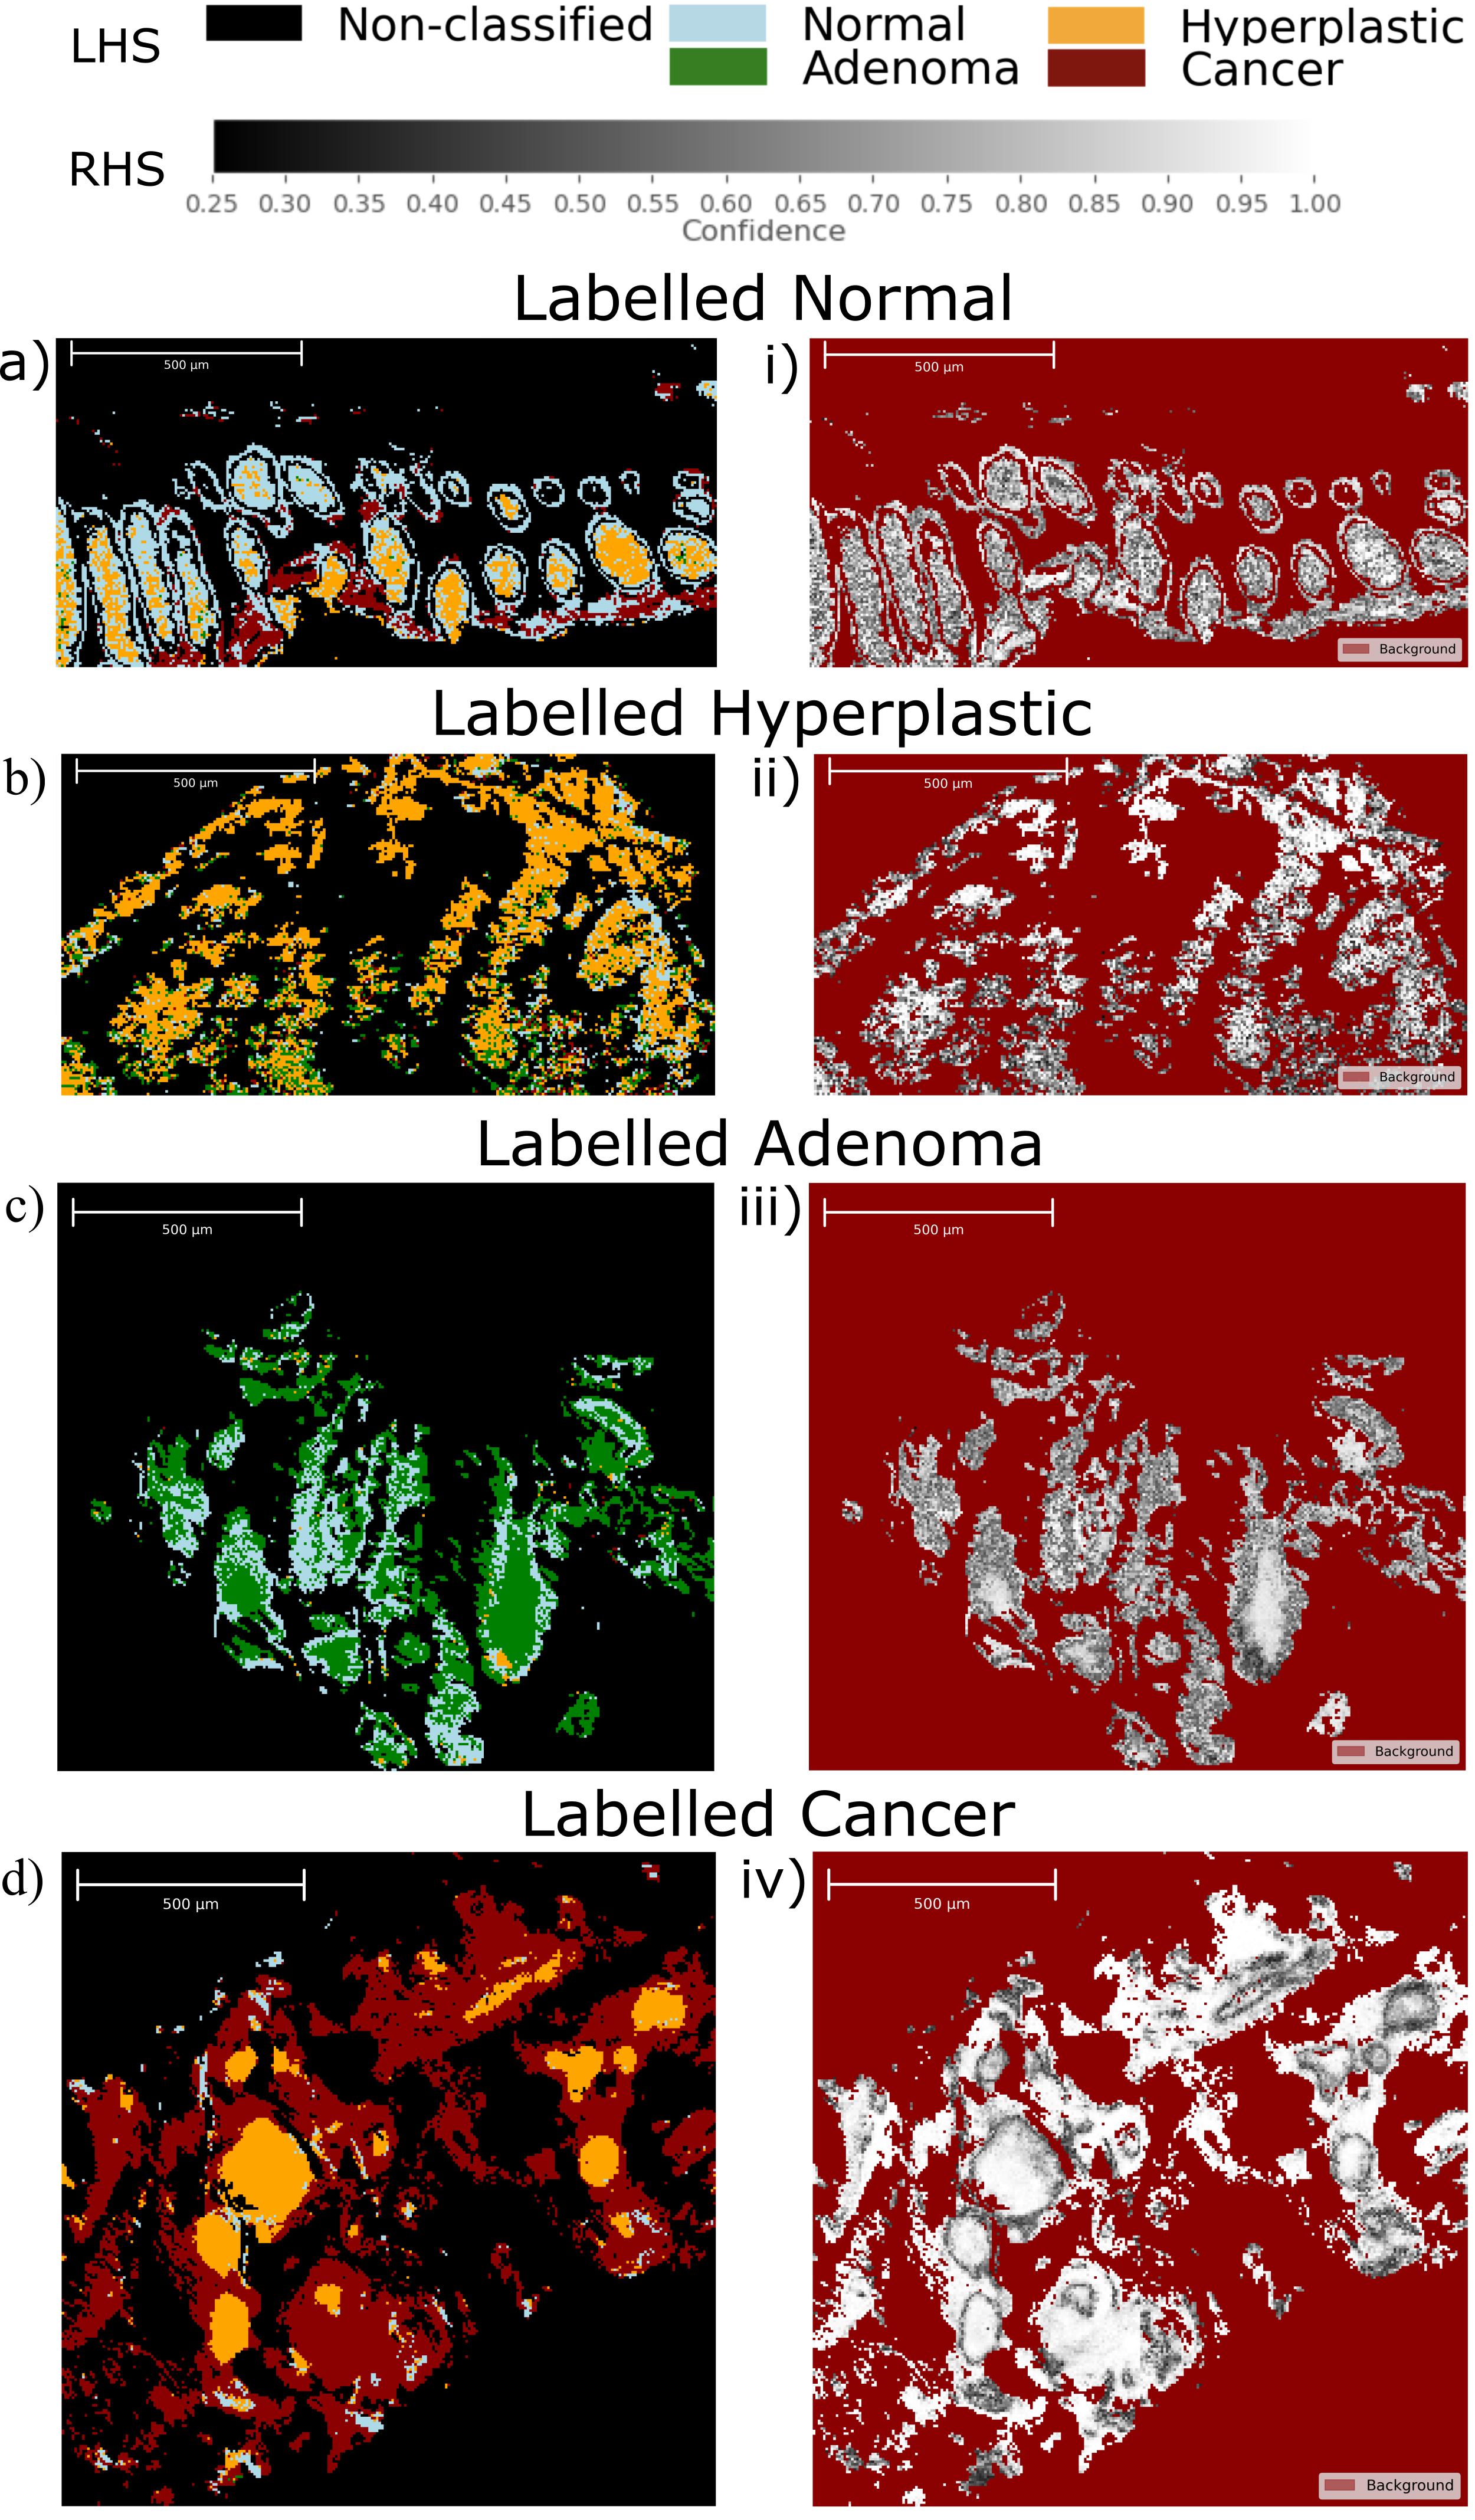
\includegraphics[width=0.8\textwidth]{Images/Confidence.png} 
    \caption{Caption} \label{fig:my-label}
\end{figure}

\begin{table}[ht] \centering \caption{XGBoost} \label{tab:xgboost}
\begin{tabular}{lcccc} \toprule Metrics & Normal & Hyperplastic & Adenoma & Cancer \\ \midrule Accuracy & $0.809\pm0.026$ & $0.826\pm0.011$ & $0.749\pm0.073$ & $0.888\pm0.055$ \\ Sensitivity & $0.490\pm0.115$ & $0.386\pm0.133$ & $0.781\pm0.055$ & $0.603\pm0.091$ \\
Specificity & $0.886\pm0.029$ & $0.911\pm0.036$ & $0.711\pm0.104$ & $0.937\pm0.057$ \\ False Positive Rate & $0.115\pm0.029$ & $0.090\pm0.036$ & $0.289\pm0.104$ & $0.063\pm0.057$ \\ \midrule \multicolumn{5}{c}{\textbf{Overall Weighted Accuracy:}
$0.565\pm0.058$} \\ \bottomrule \end{tabular} \end{table}

\begin{table}[ht] \centering \caption{SCNN} \label{tab:scnn_tpl3}
\begin{tabular}{lcccc} \toprule Metrics & Normal & Hyperplastic & Adenoma & Cancer \\
\midrule
Accuracy & $0.756\pm0.071$ & $0.801\pm0.083$ & $0.707\pm0.017$ & $0.881\pm0.070$ \\
Sensitivity & $0.739\pm0.111$ & $0.323\pm0.069$ & $0.527\pm0.071$ & $0.777\pm0.082$ \\
Specificity & $0.760\pm0.101$ & $0.894\pm0.095$ & $0.883\pm0.089$ & $0.899\pm0.072$ \\
False Positive Rate & $0.240\pm0.102$ & $0.107\pm0.095$ & $0.118\pm0.089$ & $0.102\pm0.072$ \\
\midrule \multicolumn{5}{c}{\textbf{Overall Weighted Accuracy:} $0.591\pm0.003$} \\
\bottomrule \end{tabular} \end{table}


\subsection{Explainability}
% A bit of background on why explainability is important and why it must be used in medical contexts
\subsubsection{Local Interpretable Model-Agnostic Explanations}
\begin{figure}[htbp]
  \centering
  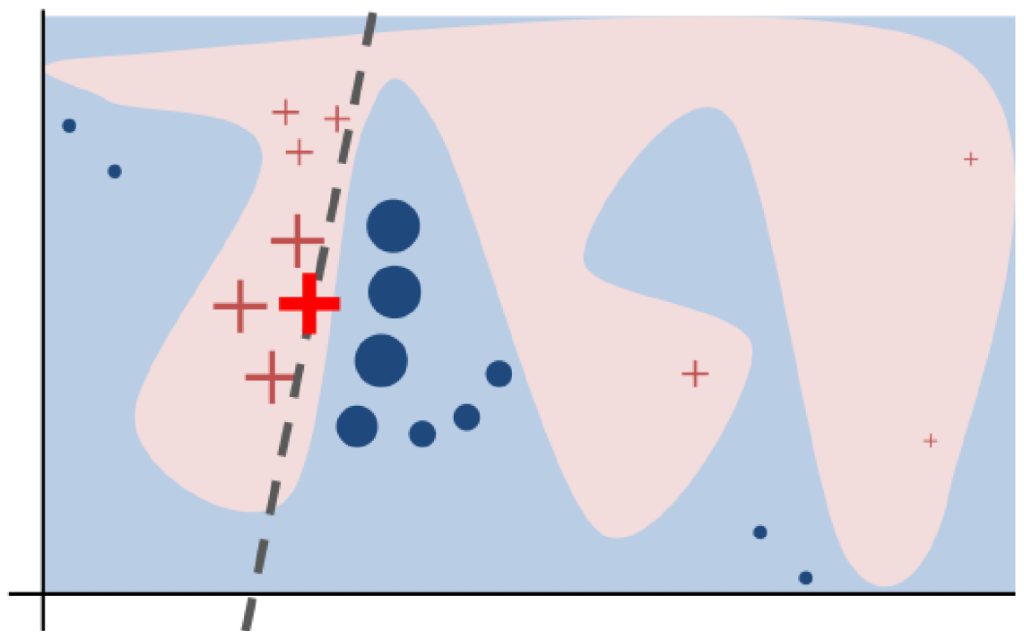
\includegraphics[width=0.8\textwidth]{Images/lime_explanation.png}
  \caption{From \cite{ribeiro_why_2016}}
  \label{fig:my-label}
\end{figure}

\begin{figure}[htbp]
  \centering
  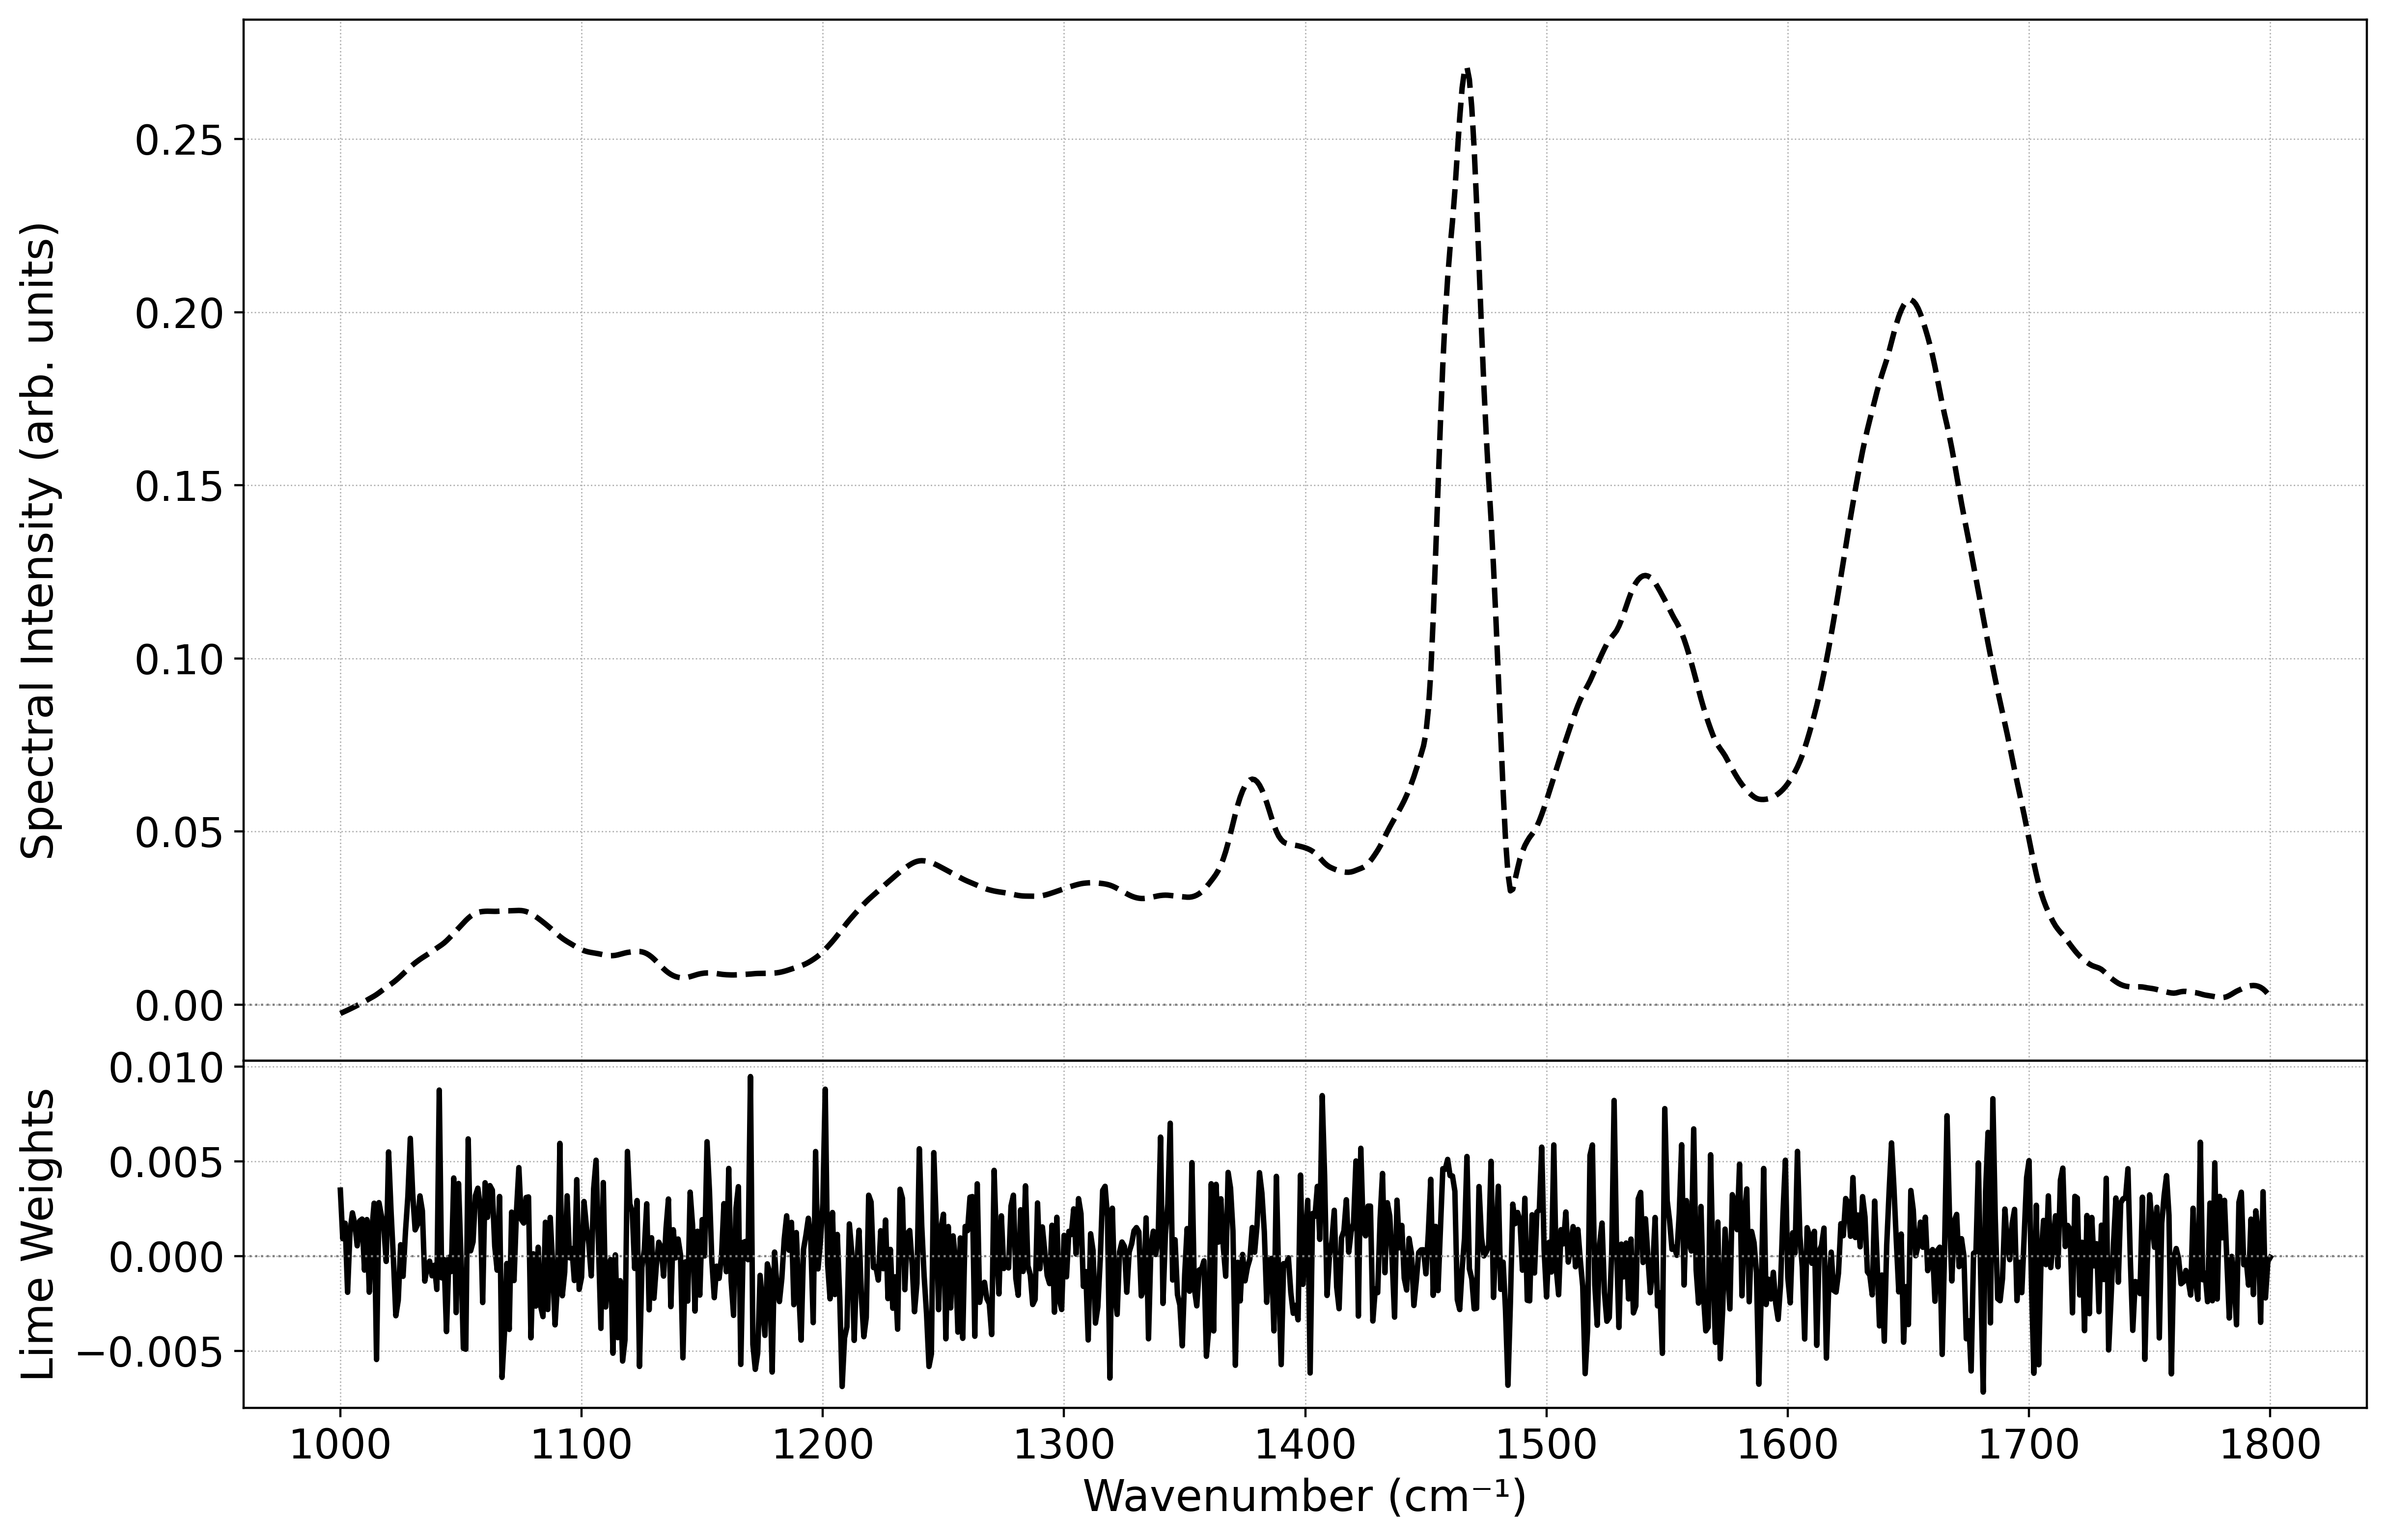
\includegraphics[width=0.8\textwidth]{Images/lime_weights_example.png}
  \caption{Caption}
  \label{fig:my-label}
\end{figure}

\subsubsection{CRIME}
\begin{figure}[htbp]
  \centering
  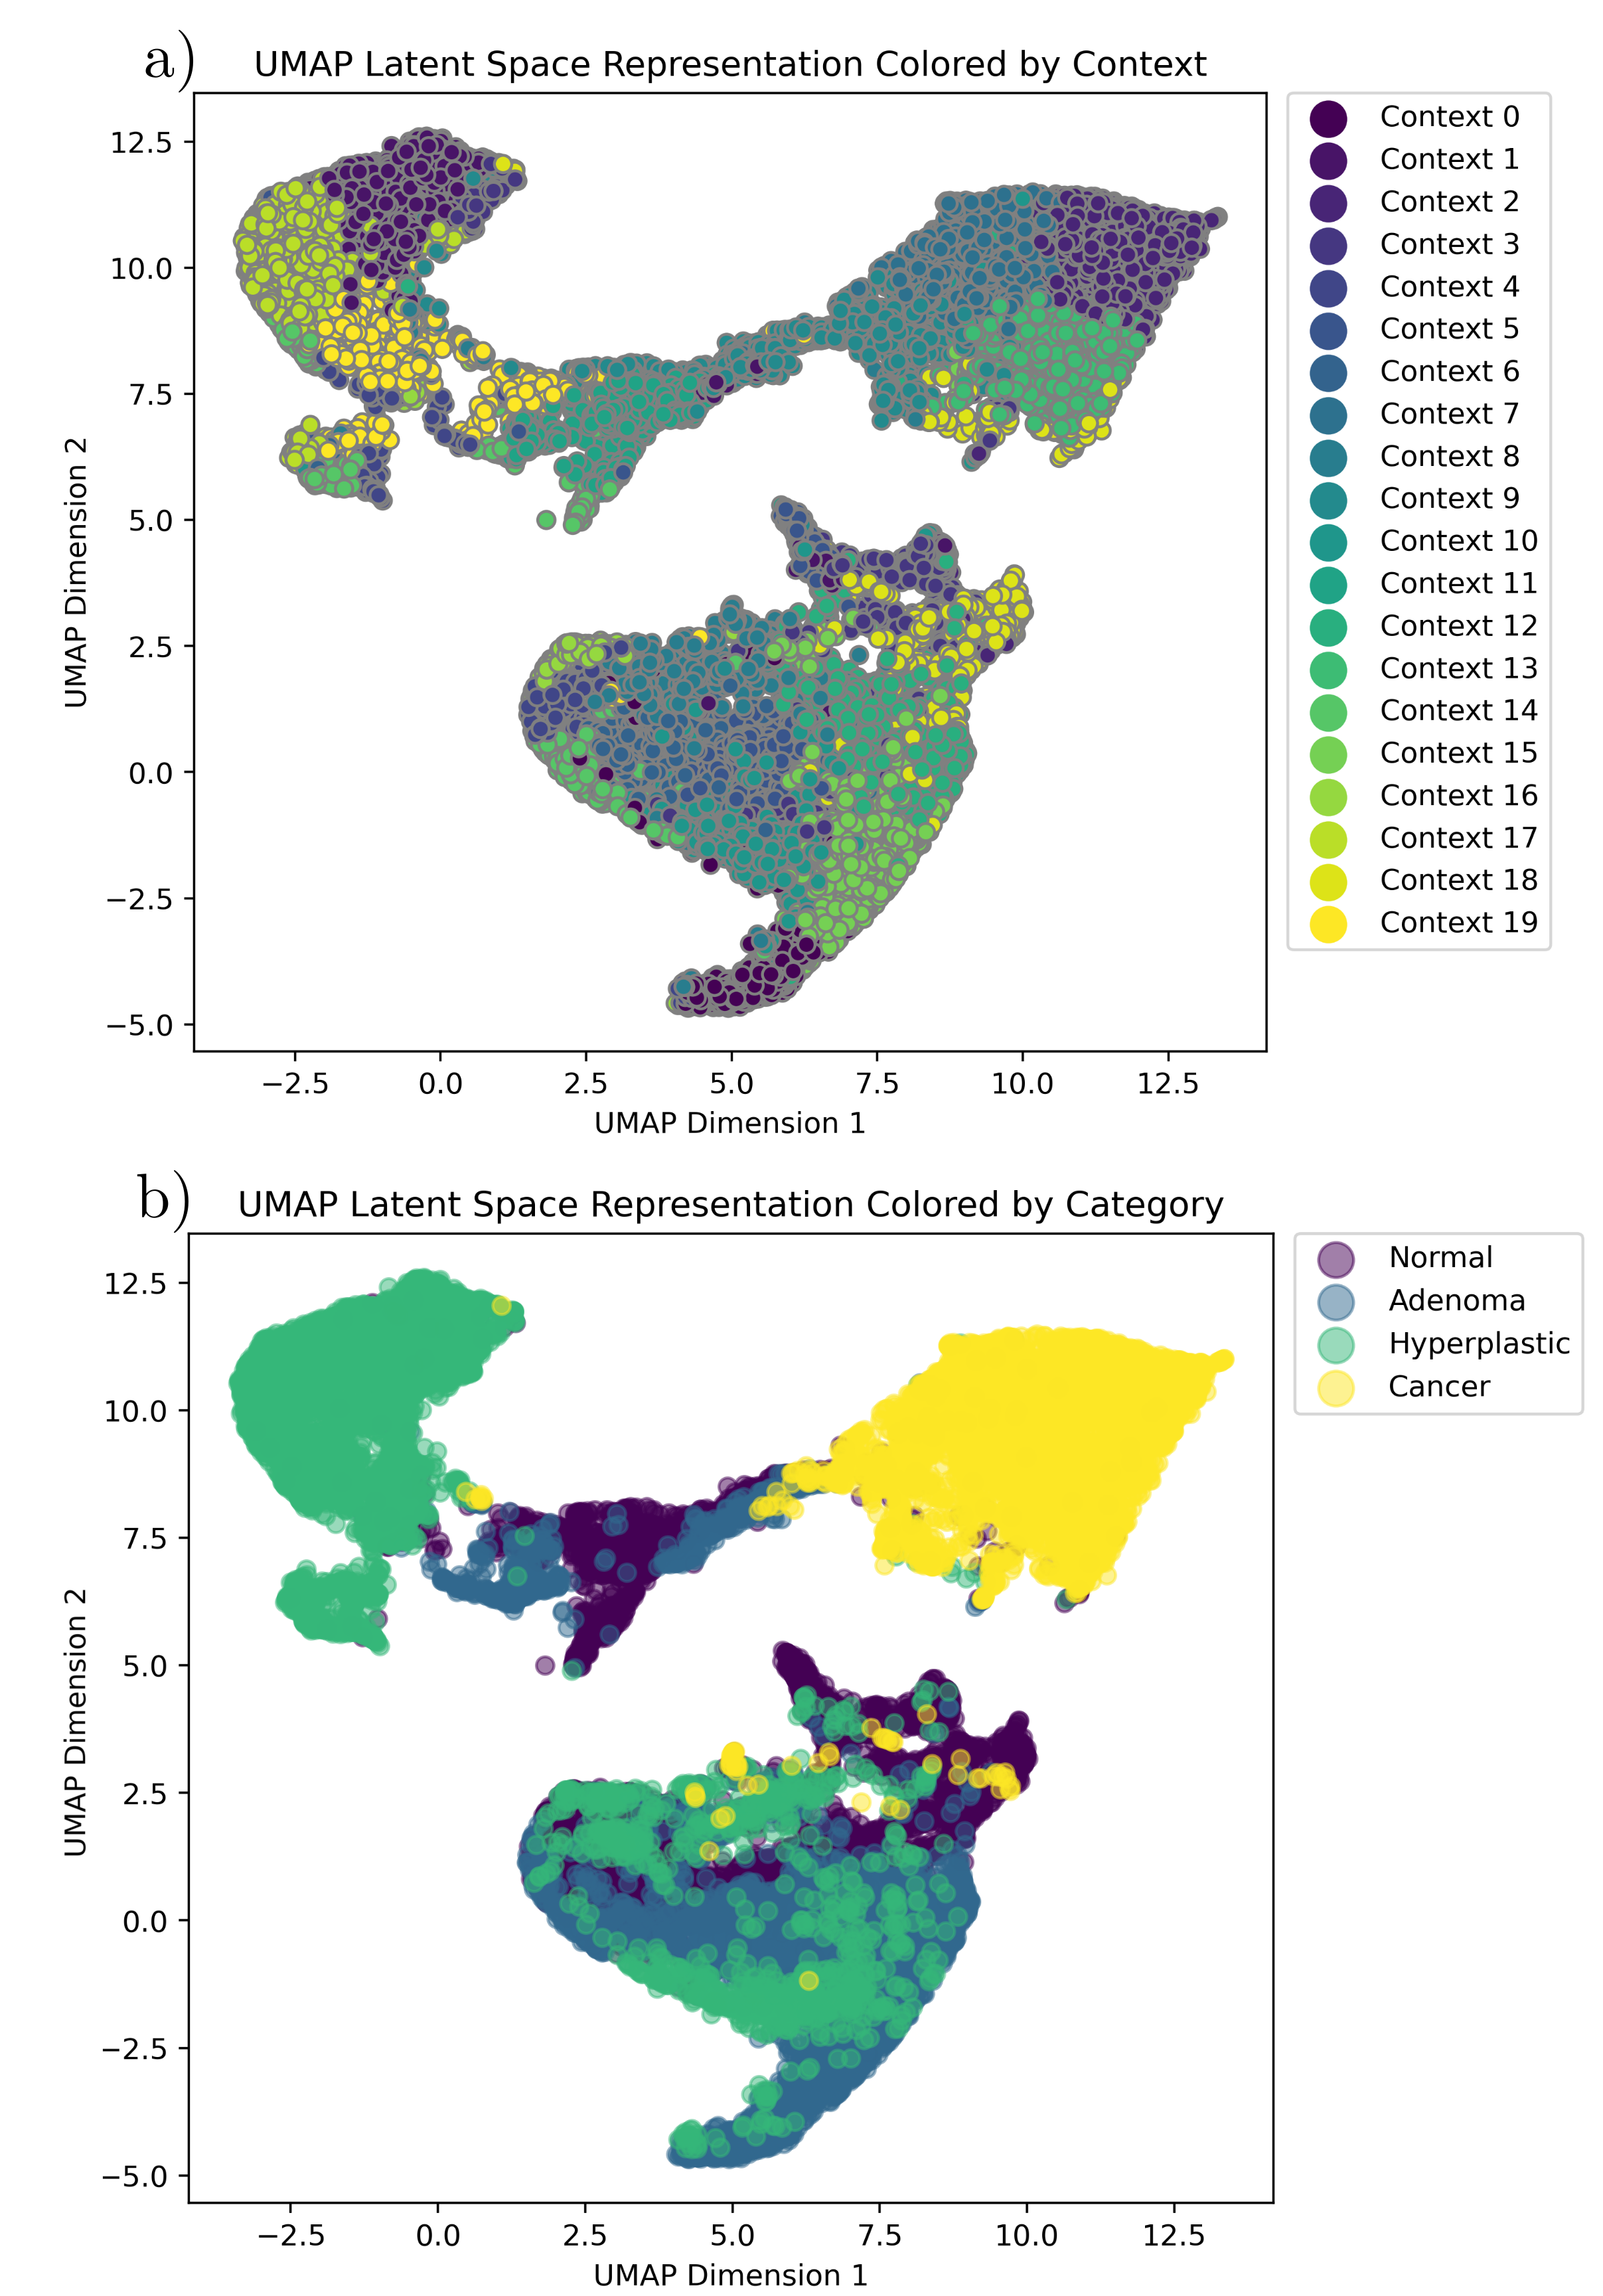
\includegraphics[width=1\textwidth]{Images/crime_umap.png}
  \caption{Caption}
  \label{fig:my-label}
\end{figure}
\subsubsection{VAE Methods}

\begin{figure}[htbp]
  \centering
  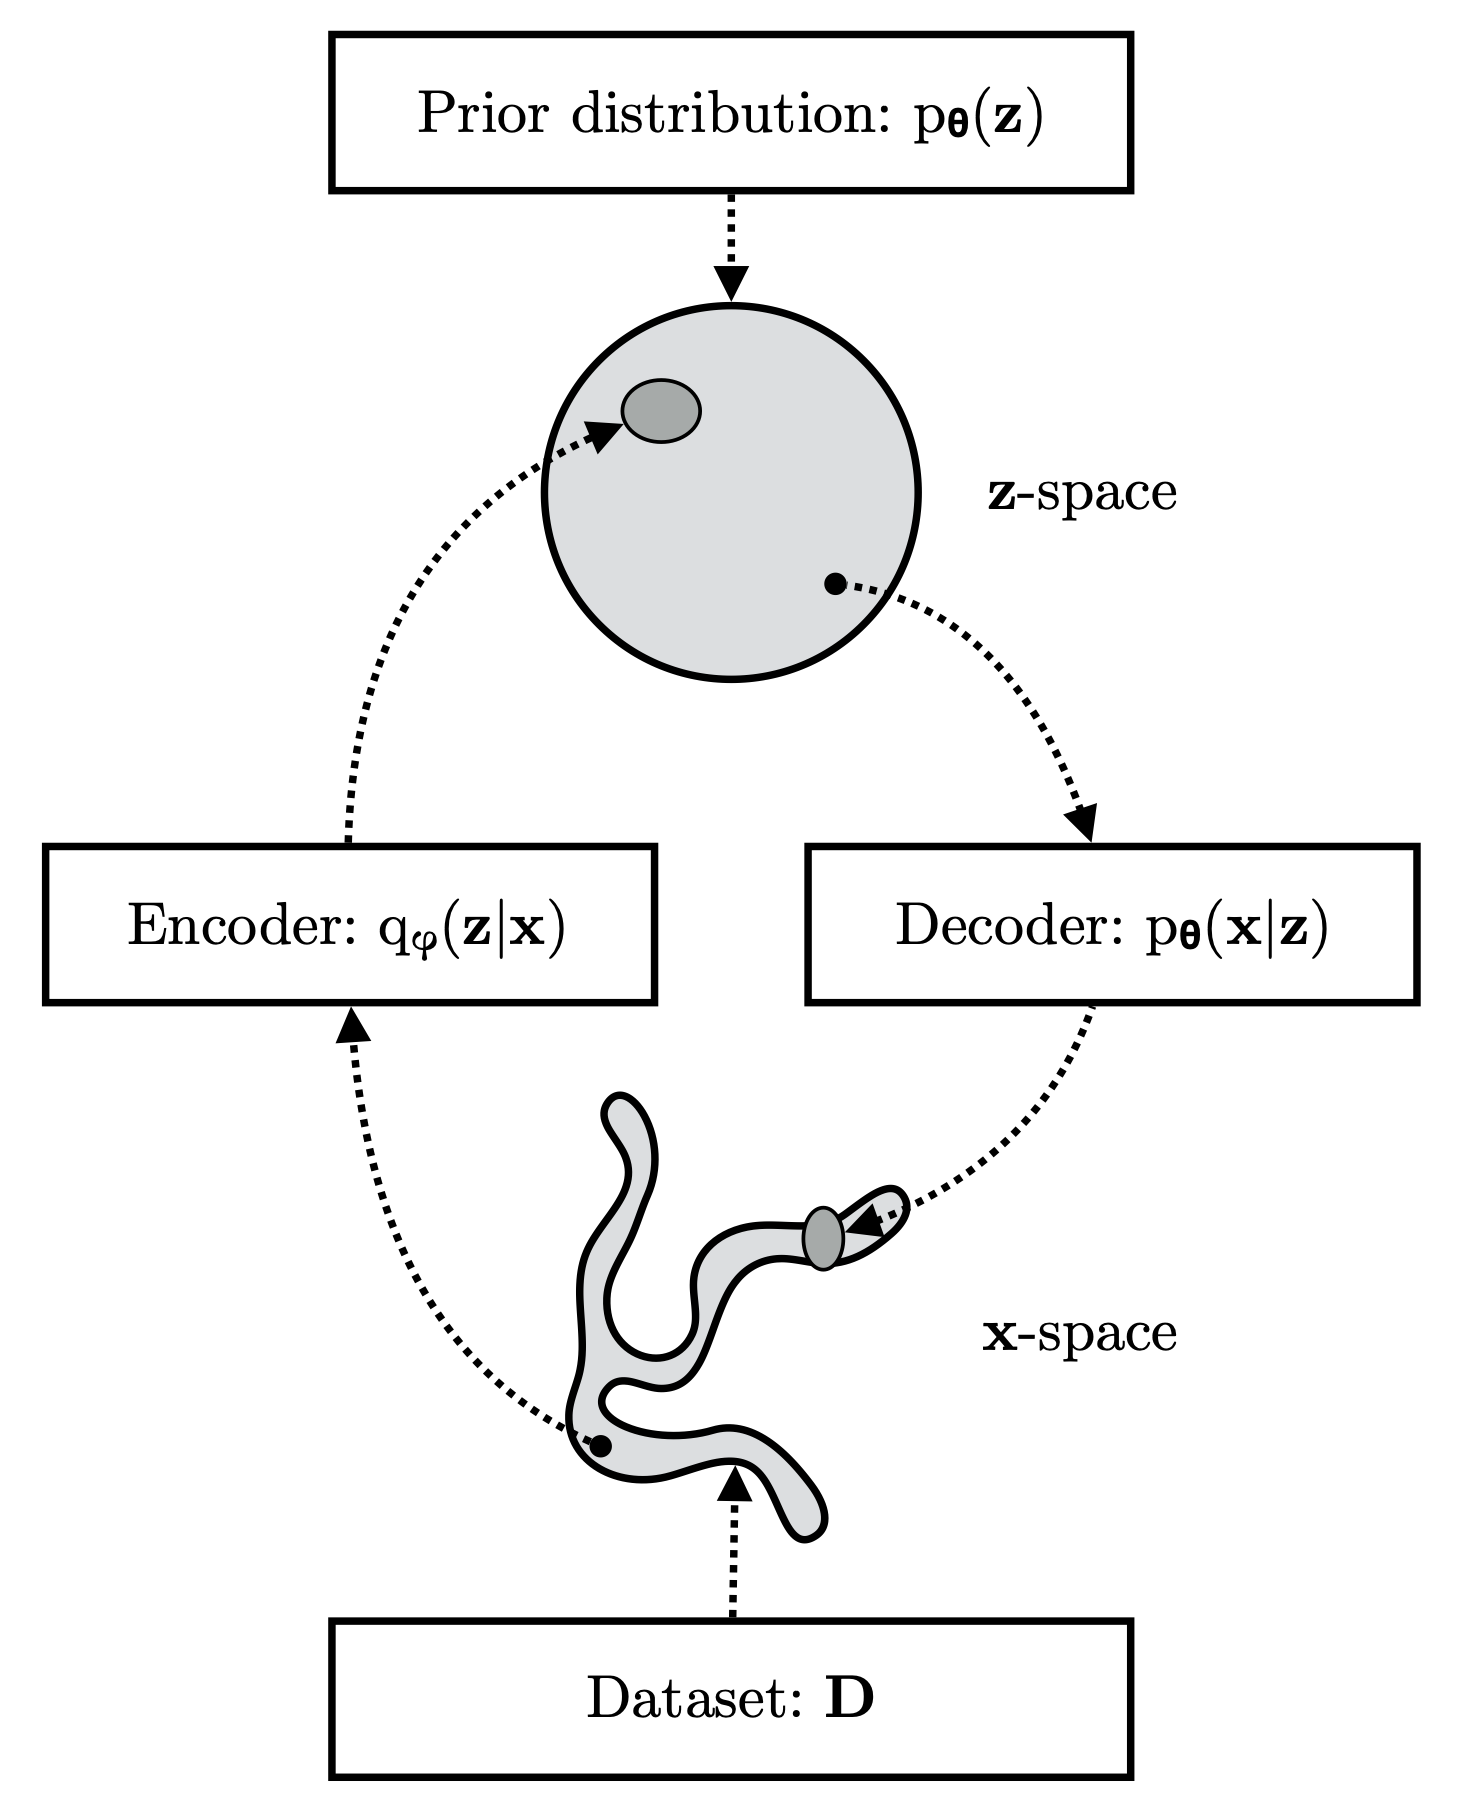
\includegraphics[width=0.8\textwidth]{Images/VAE_overview.png}
  \caption{From \cite{kingma_introduction_nodate}}
  \label{fig:my-label}
\end{figure}

\paragraph{Clustering VAE Approaches}

\begin{figure}[htbp]
  \centering
  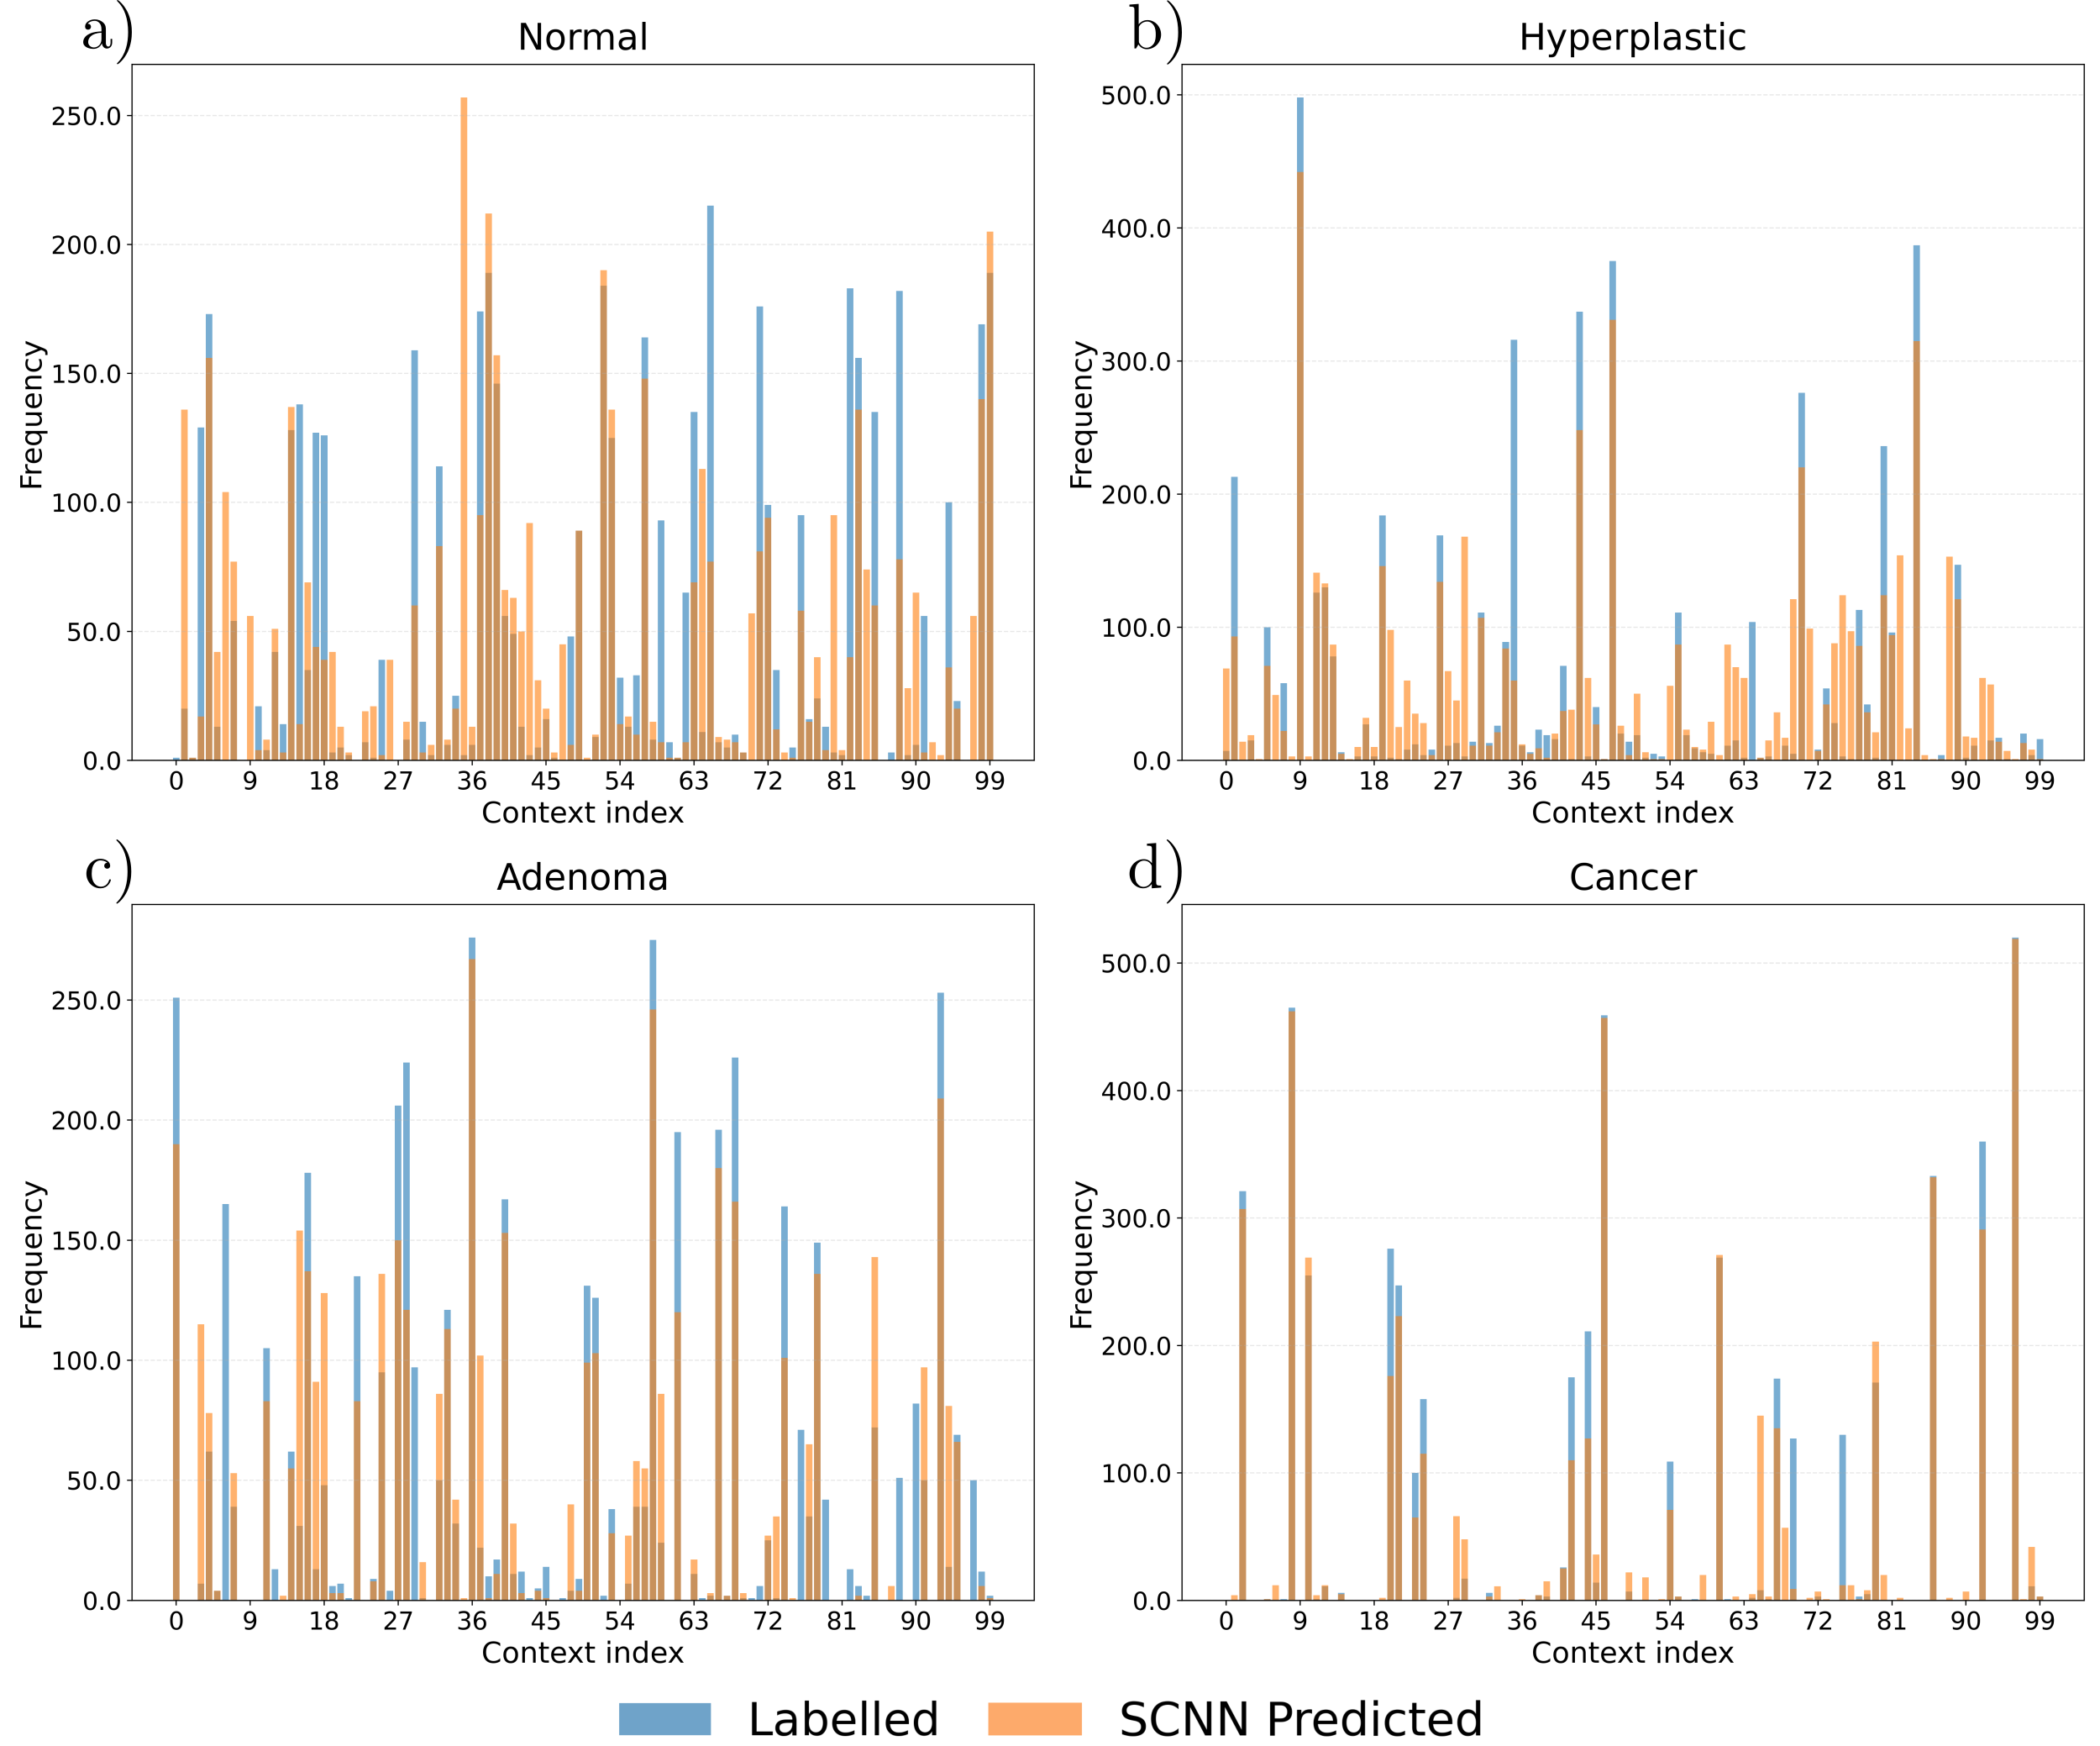
\includegraphics[width=1\textwidth]{Images/crime_groupings_by_category_100.png}
  \caption{Caption}
  \label{fig:my-label}
\end{figure}

\begin{figure}[htbp] 
    \centering 
    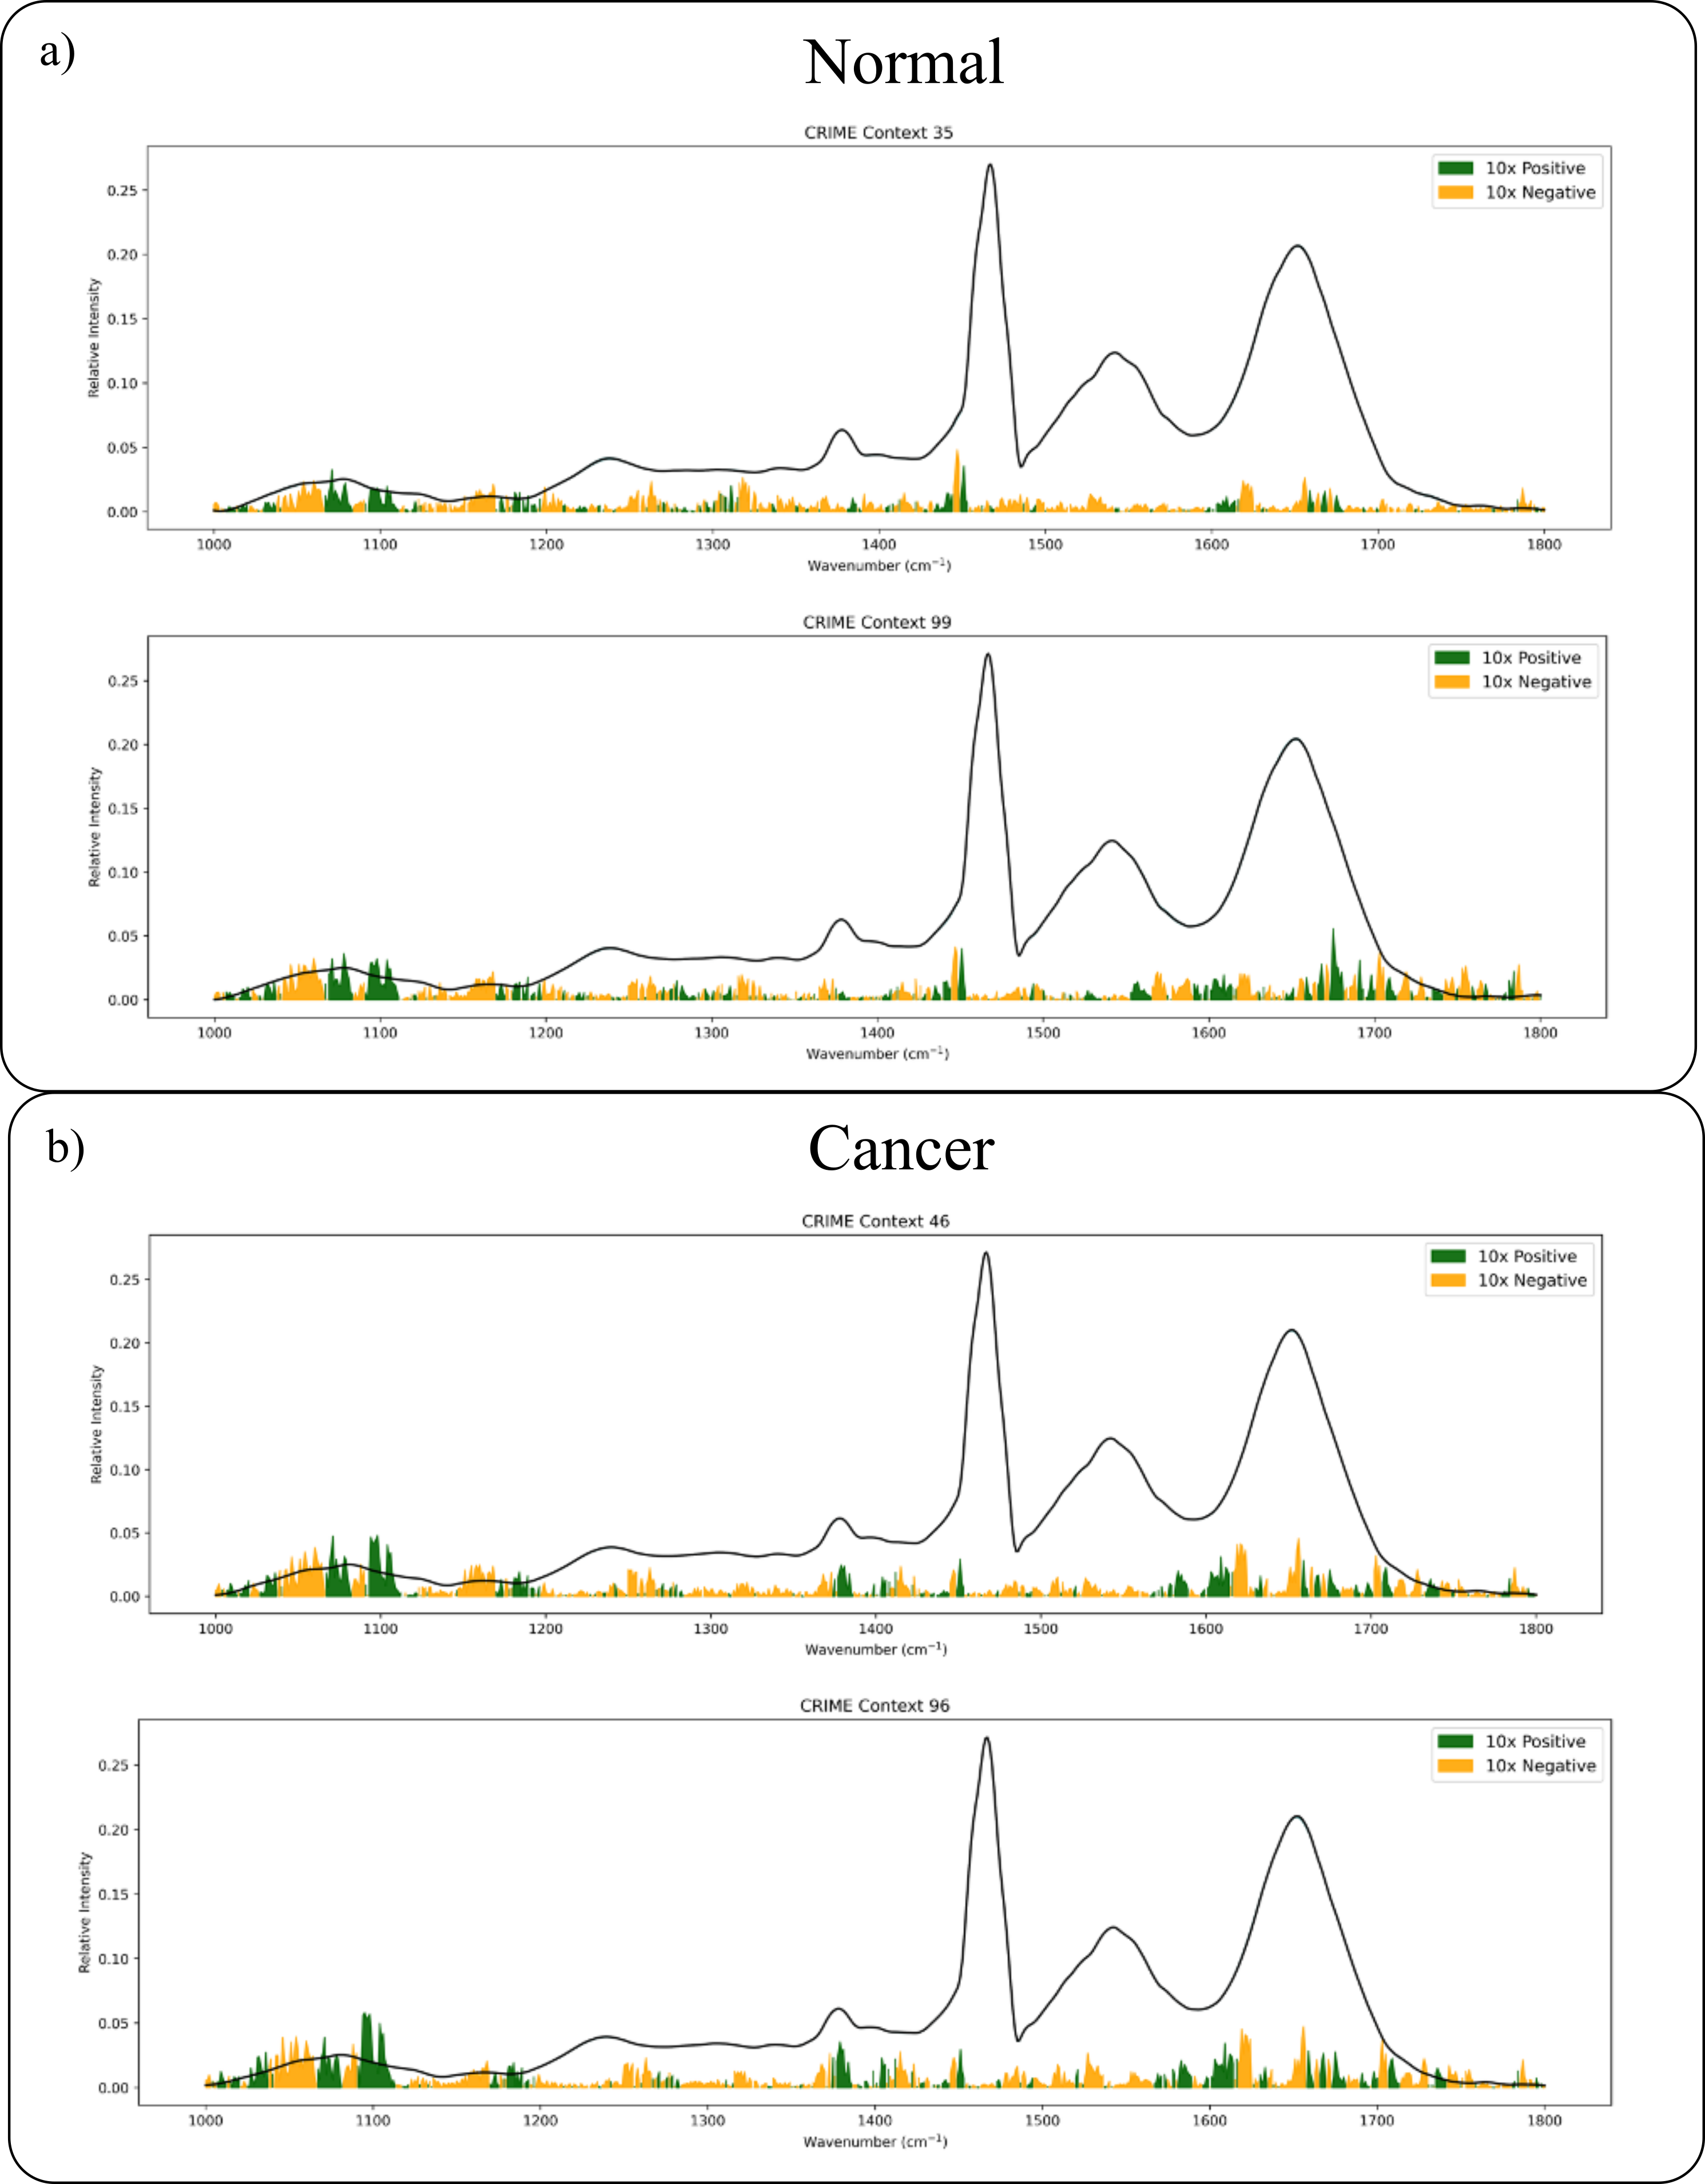
\includegraphics[width=1\textwidth]{Images/crime_lime_plots.png} 
    \caption{Caption}
\label{fig:my-label} \end{figure}

\begin{figure}[htbp]
    \centering
    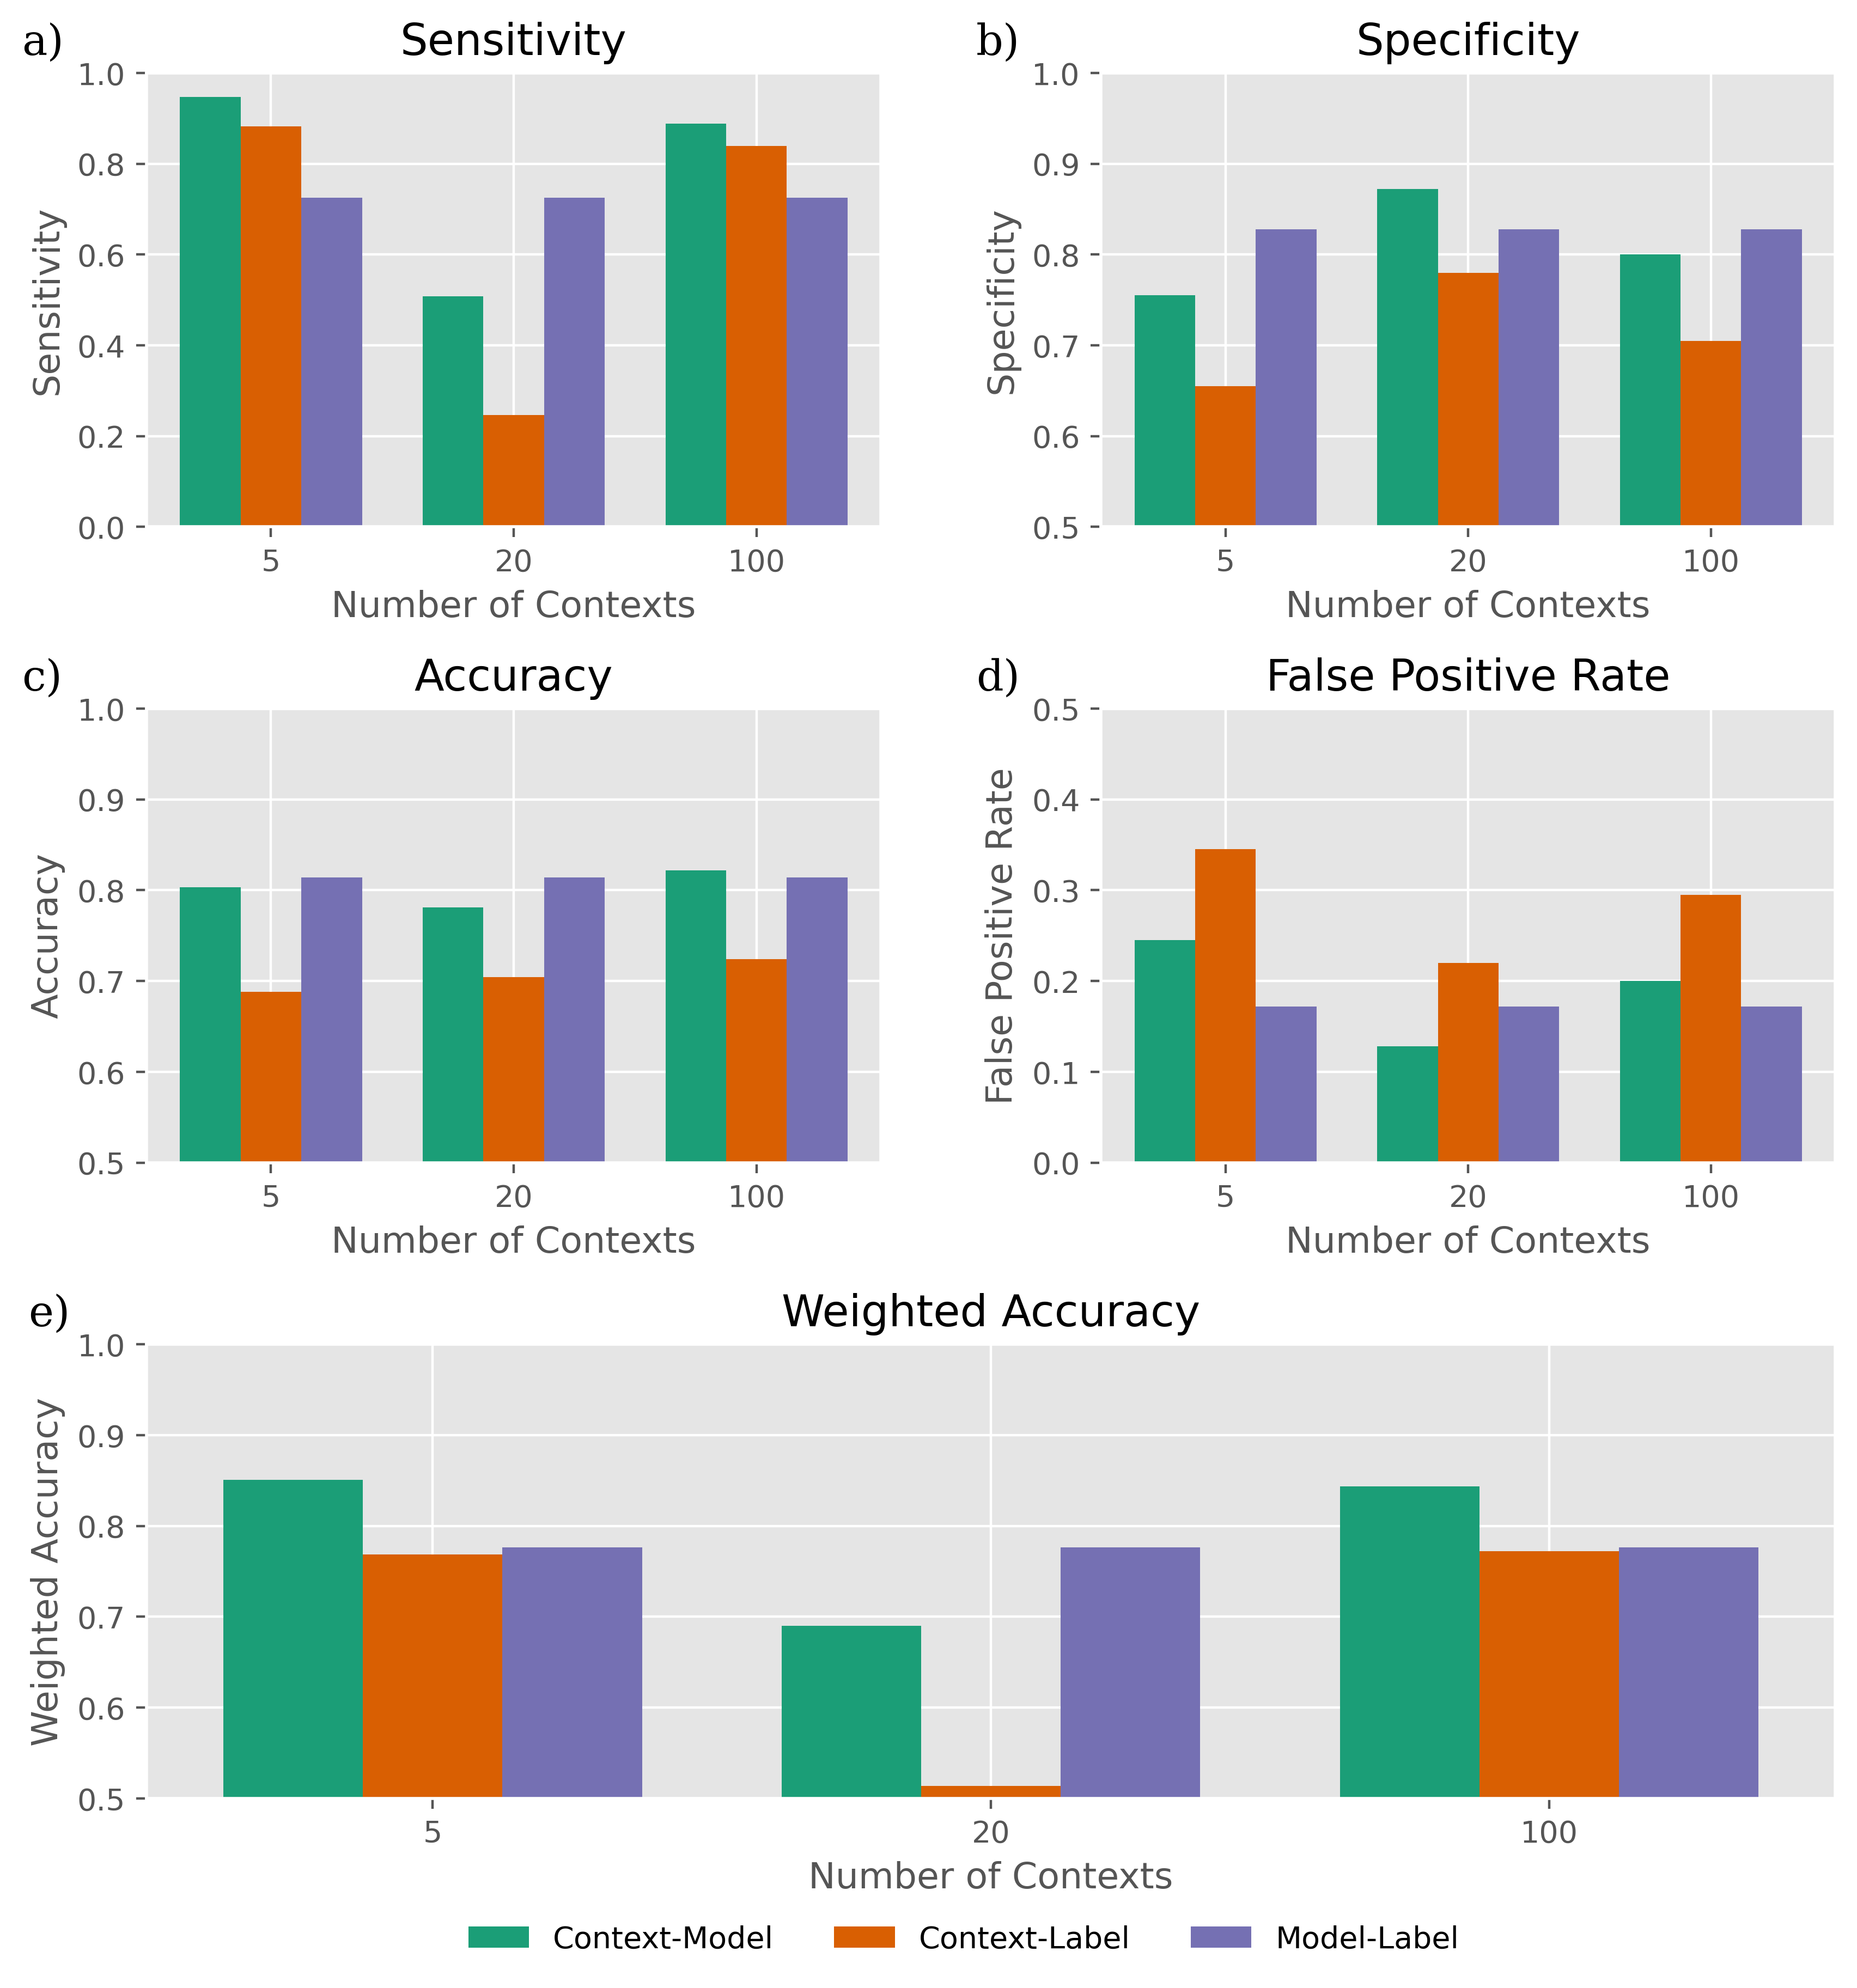
\includegraphics[width=1\textwidth]{Images/context_model_metrics.png}
    \caption{Caption} \label{fig:my-label} 
\end{figure}

\paragraph{Logic Explained Networks}